\documentclass{article}
\usepackage[left=2cm, right=2cm, top=1cm]{geometry}
\usepackage[utf8]{inputenc}
\usepackage{amsmath}
\usepackage{enumitem}
\usepackage{float}

\title{Hyperspectral Imaging Biodiversity}
\author{Hannah Gallagher}
\date{October 13th, 2024}

\usepackage{natbib}
\usepackage{graphicx}

\begin{document}

\maketitle

\section{Introduction}

%Convolution 
%Eigenvalues Eigenvectors 
%Discrete fourier transform 
%Continuous transform 
%Vector basis 
%Circulant matrix
%Euler relation



% Hot keys to remember: command / on a mac comments highlighted code in and out.
%Nugget the snowman wishes you good luck on your research!

%\begin{figure}[h!]
%\centering
%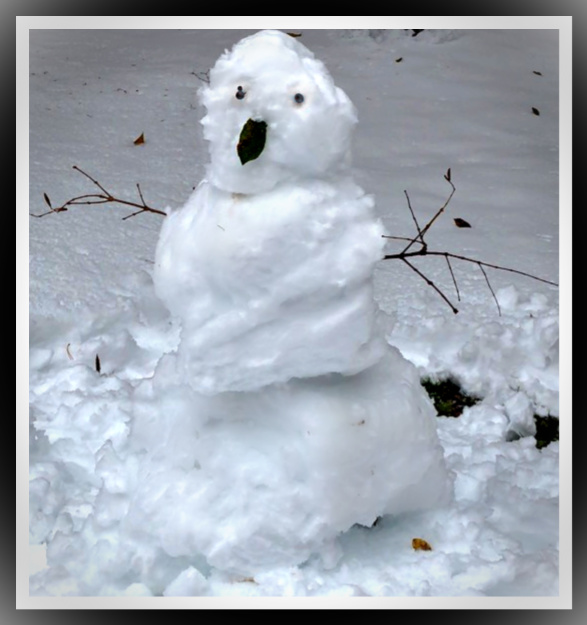
\includegraphics[scale=1]{Nugget.jpg}
%\caption{Nugget the Snowman}
%\label{fig:Nugget}
%\end{figure}

\section{Given Information, Key Terms, and Things to Remember} 
\begin{itemize}
\item Hyperspectral Imaging
\item ENVI
\item Radiance
\item https://scienceandtechnology.jpl.nasa.gov/dr-marc-simard
\item Parameterization of stuff and that NASA problem 7 on pset 2
\item Solid Angle 
\item All the different definitions around radiance, irradiance, radiant intensity etc.
\item 4PIX
\item Edge Detection
\item Global Warming
\item Salt Marshes protect ecosystems
\item LiDAR shows more fine details


% \begin{figure}[h!]
% \centering
% 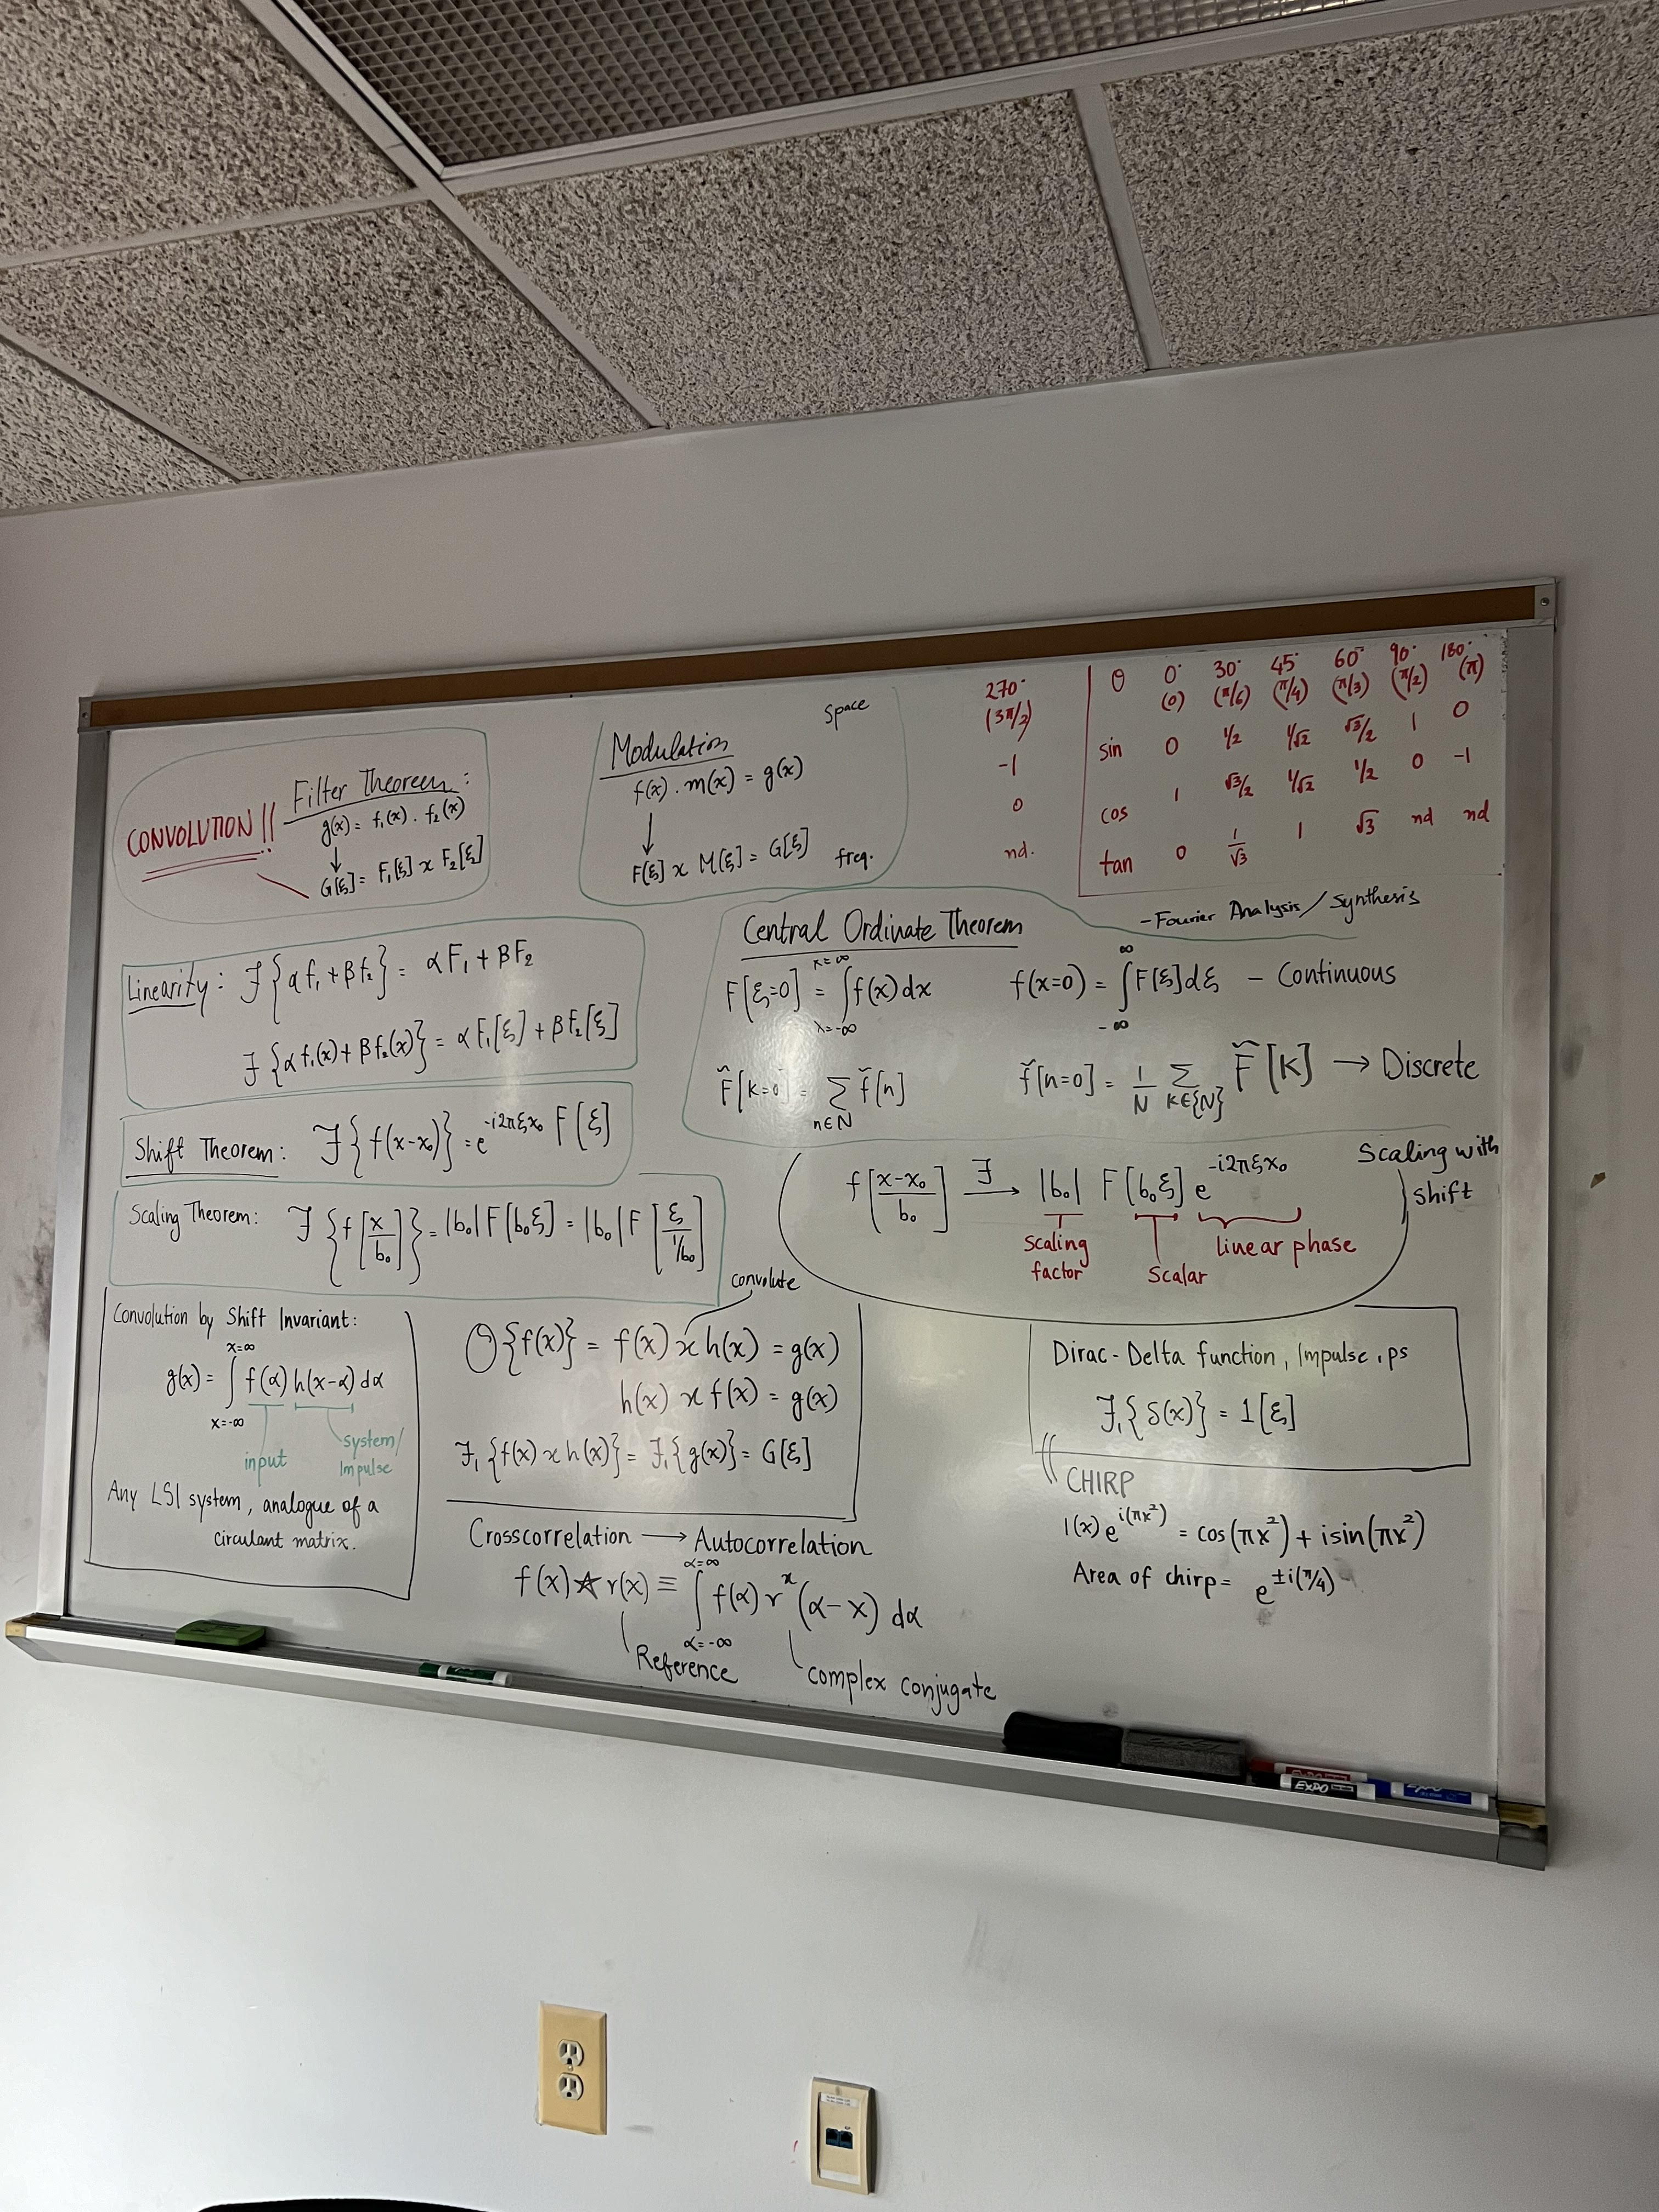
\includegraphics[scale=.20]{Fourier/unnamed.jpg}
% \caption{Easton Syllabus}
% \label{fig:Snowman4}
% \end{figure}


 
\end{itemize}

\clearpage

\section{Day by Day}

\subsection{October, 2024}
(Beginning stages in another document along with weekly GRIT meetings are in a google doc.)
Nayma wrapping up research and explaining how to use the dat files and open shape files in ENVI as they all need to be present to view the file. 

\subsection{November 8th, 2024}
Finally achieved the mosaic image in ENVI during the research meeting. Asked about a hard drive to borrow.



\subsection{November 13th, 2024}
Research meeting after the second Fourier exam. Received the hard drive to borrow as it was okayed to be cleared.

\subsection{November 15th, 2024}
Week frees up a little bit and made plans to read more papers on hyperspectral imaging, red edge, and ENVI over the weekend. Quick check in with Dr. Bachmann to ask about possible meeting times. Grant due Monday for Dr. Bachmann so Tuesday meeting planned. (Will also have to be quick).

\subsection{November 21st, 2024}
Undergraduate research presentation for AWM and PiRIT. Practiced public speaking and speaking about research. 

\subsection{November 22nd, 2024}
Bowling with Pure Physicists.    

\subsection{November 23rd, 2024}
Went to High Acres Nature Area. (HANA) 

Studied how I could learn about tree health in marshes from the ground level as everything I'm working in is too small. Need a broader idea to get started. 

See end of document to see pictures from the tree study. 


\subsection{November 26th, 2024}
Studied and read the Radiometry textbook 2-5 again. 

\subsection{November 27th, 2024}
Had the idea to use the human vision review model to do this lit review. Read a few papers that were review papers, but they really only spoke on different software. Looked over the lab data and that may help in the future knowing those fundamentals. 



\subsection{November 28th, 2024}
Read more papers about software, such as random forest, not very insightful as I have already used random forest in past research. Anything done with machine learning was glossed over.  

\subsection{November 29th, 2024}

(Early Morning) Application of leaf multispectral analyzer in comparison to hyperspectral device to assess the diversity of spectral reflectance indices in wheat genotypes: Sunlight is important in analyzes the health of an ecosystem as it is needed for photosynthesis. 
Plant Senescence Reflectance Index. 

(Noon) Read Radiometry Textbook Chapters 7-10 again on the drive home from Thanksgiving. Various relevance to Radiometry as Photometry is not the focus. 

Crop yields paper and fertilizer levels differences\\
(Evening) 10 year high school reunion. Spoke about research and had a few ideas for research topics more relating to human vision. 
Went to bed early and was too tired to look at anything. 


\subsection{November 30th, 2024}
Spoke about research with neighbors at annual Christmas Tree party. Practice for explaining topics and thoughts. Importance of detection of dry leaves for fires as wind blew the leaves towards the fire. Browsed papers when home about research papers relating to campfire smoke in eyes and detectability in satellite, hyperspectral imaging etc. Thought more about Volcanic atmospheric conditions. 


\subsection{December 1st, 2024}
Spent the early morning watching Radiometry lectures again from the midterm to Thanksgiving. Took notes in LaTeX on what was mentioned and emphasized in each lecture. Looked through the homework again. Found the relevant lecture that mentioned all of the important practice problems for the homework.

Continued to work on the lab. Found relevant lectures pertaining to that. 

Continued  to keep up with Dr. Bachmann Google Scholar notifications. Read those papers and then extrapolated from the related OSA papers in one of the beach studies from 2015. Found a study on the development of white radishes in China which require ample nitrogen which relates to Nayma's work. 

Browsed ENVI's abilities and help menu. Downloaded more photos. 

My dad wanted a marble ball bee water feeder for Christmas and I looked up some papers on how it worked. Apparently bees see in UV light. I already know a lot about bees so that could be an avenue. 

\subsection{December 2nd, 2024}

Early Morning: Read papers on hyperspectral and LiDAR imaging of bee and floral biodiviersity.

QUESTION: 
How can Lauren detect the snails she's studying for their biodiviersity in the marshes? Aren't they too small? They're most likely brown so in a muddy environment they probably blend in. Could she simply be looking for the plants or looking at different pictures that are closer to the ground?

Plan: 
Continue to work on Radiometry Lab and Homework. Do easy questions for Fourier. Submit final draft outline for Human Vision. Listen to more papers while grading etc. 

Tomorrow: Finish up Fourier homework. Work on Lab and ask questions. 

Wednesday: Go to seminar to ask questions and work on Radiometry Lab. 


% \[
%     V= \frac{4}{3} \pi (b^3 + c^3 + f^3)    
% \]


% \[
%     V= \frac{4}{3} \pi (2^3 + 1.75^3 + 1^3)    
% \]

% \[
%     V= \frac{4}{3} \pi (8 + 5.359375 + 1)    
% \]

% \[
%     V= \frac{4}{3} \pi (8 + 5.359375 + 1)    
% \]

% \[
%     V= 19.1458333 \pi \; ft^3  
% \]



% \section{Question 3}        


% From before, 
% \[
%     V= \frac{4}{3} \pi (r^3)  
% \]

% Let C (t)= Volume of the center sphere at time t. 

% At t= 8 min. 


% \[
%     C = \frac{4}{3} \pi ((.75+.25(t-7))^3)  
% \]

% \[
%     \frac{dC}{dt}= \frac{4}{3} \pi ((.75+ \frac{8-7}{4})^2)\frac{dt}{dt} * (\frac{3}{4}) 
% \]
% \[
%     \frac{dC}{dt}= \pi ((.75+ \frac{t}{4})^2)
% \]

% \[
%     \frac{dC}{dt}= 4\pi (r(t))^2 * r'(t)
% \]

% \[
%     \frac{dC}{dt}= 4\pi (1)^2 * \frac{1}{4}
% \]

% \[
%     \frac{dC}{dt}= \pi \; \; \frac{ft^3}{min}
% \]

\section{Math Needed}
\subsection{Trig Identities}
\begin{equation}
    cos(\theta)= \frac{e^{i \theta}+e^{-i \theta}}{2}
\end{equation}

\begin{equation}
    sin(\theta)= \frac{e^{i \theta}-e^{-i \theta}}{2i}
\end{equation}
Don't forget to remember your adding exponents when their bases are being multiplied by each other!
\begin{equation}
    sin(\theta)= cos(\theta - \frac{\pi}{2}) 
\end{equation}
Never forget good old SOH CAH TOA. 
He has thrown in a nice small angle approximation before as well. 


\subsection{Reflectance}

\subsection{BRDF}





%\begin{figure}[h!]
%\centering
%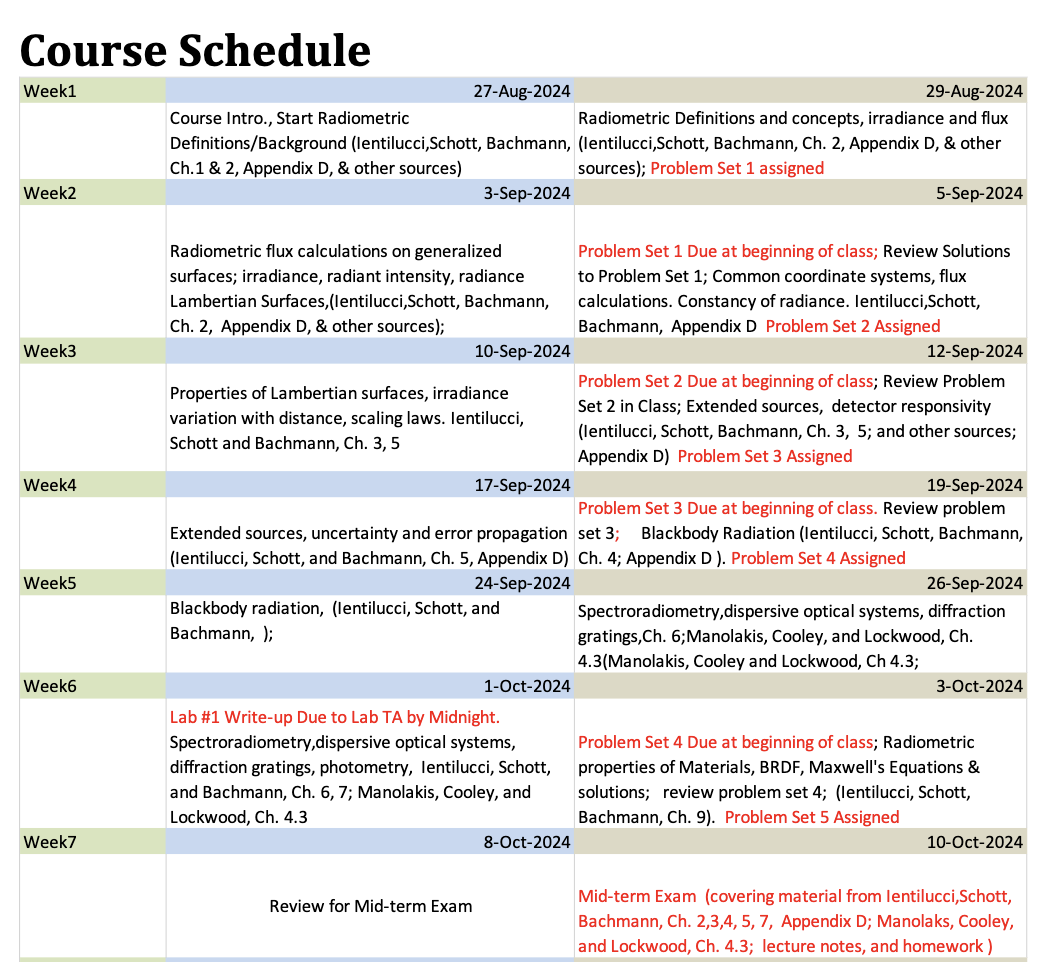
\includegraphics[scale=.95]{Radiometry/Week1/Notes/Syllabus.png}
%\caption{Course Syllabus: He goes through this pretty thoroughly, except that %we did not get to Week 6. The exam is on 2,3,4,5, and 6.}
%\label{fig:Snowman3}
%\end{figure}


\section{Equations}



%\subsection{The Grating Equation}
%Sometimes the given information is in number of grooves or lines per milimeter: lpm 
%$d_{mm} = \frac{1}{lpm}$
%\begin{equation}
%    \Gamma_{Tot}=d(sin \theta_{i} + sin \theta_{r}) = \frac{l}{N}(sin \theta_{i} + sin \theta_{r}) = m \lambda
%\end{equation}
%Where m =0,1,2,3,...

\section{HANA Tree and Marsh Study}
\clearpage
More pictures are available and in the repository of this LaTeX file. 
\begin{figure}[h!]
\centering
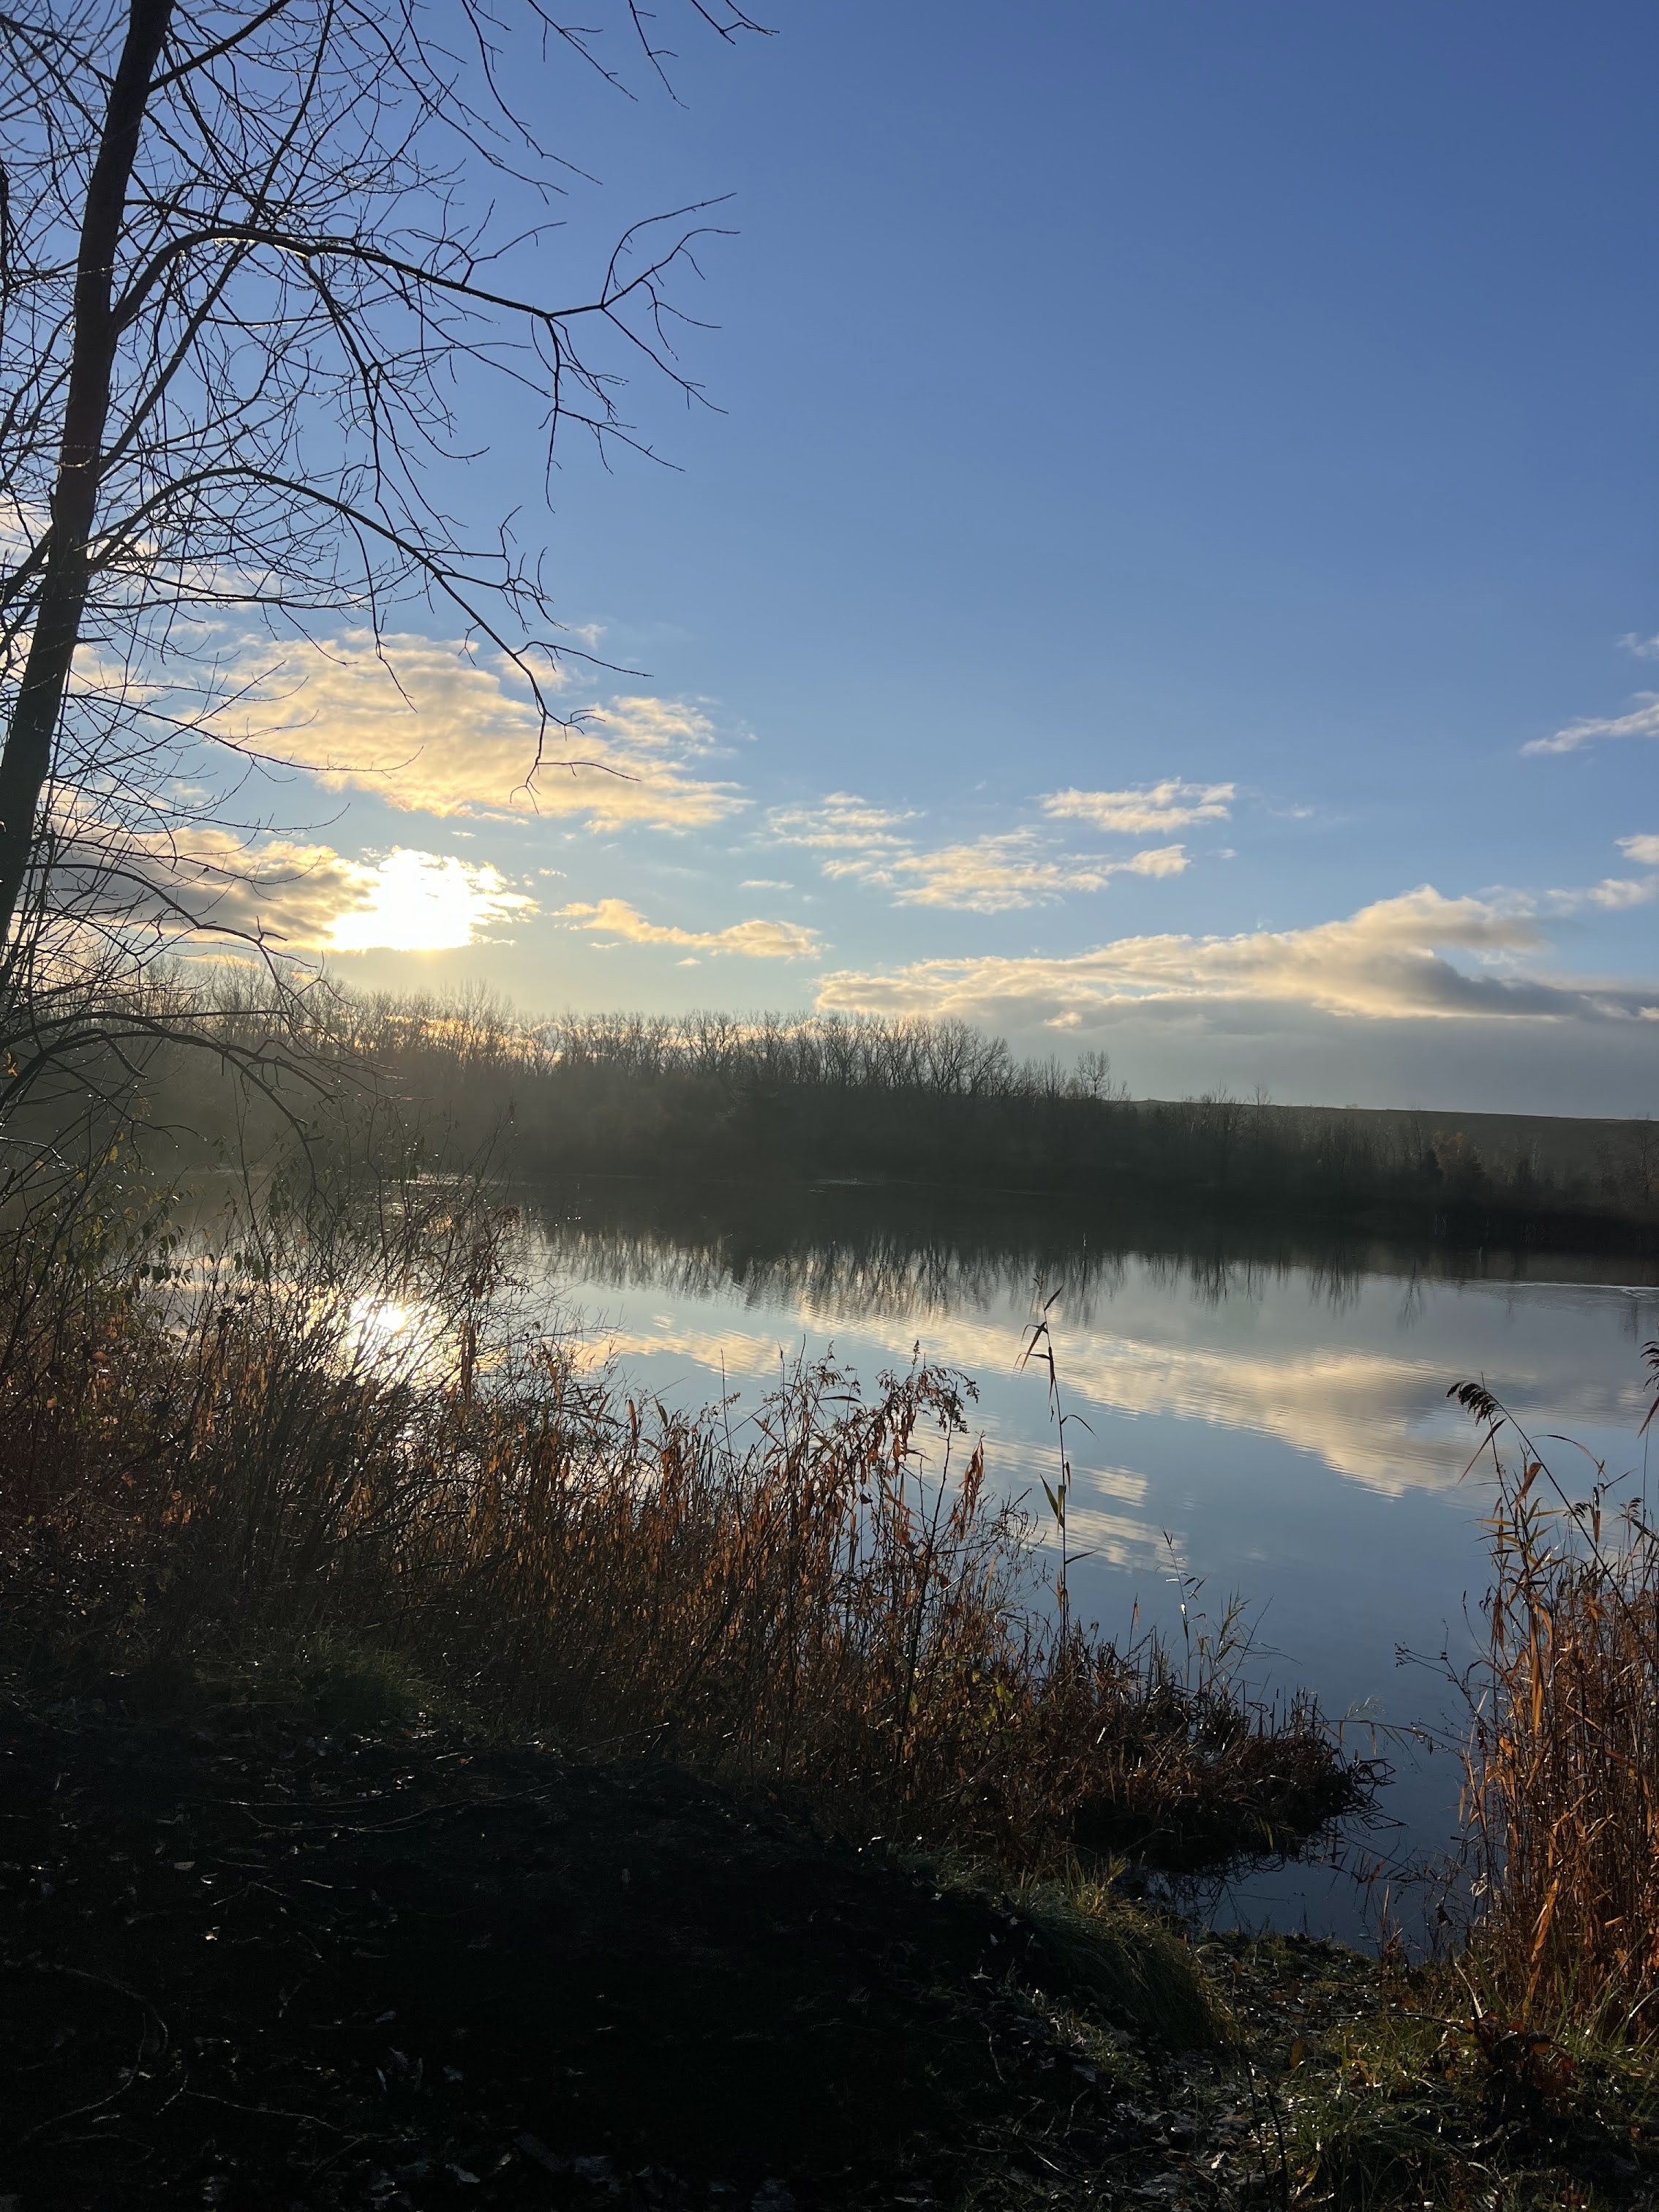
\includegraphics[scale=.1]{Research/HANA/NOV2024/IMG_9791.JPG}
\caption{HANA Tree Study}
\label{fig:HANA}
\end{figure}



\begin{figure}[h!]
\centering
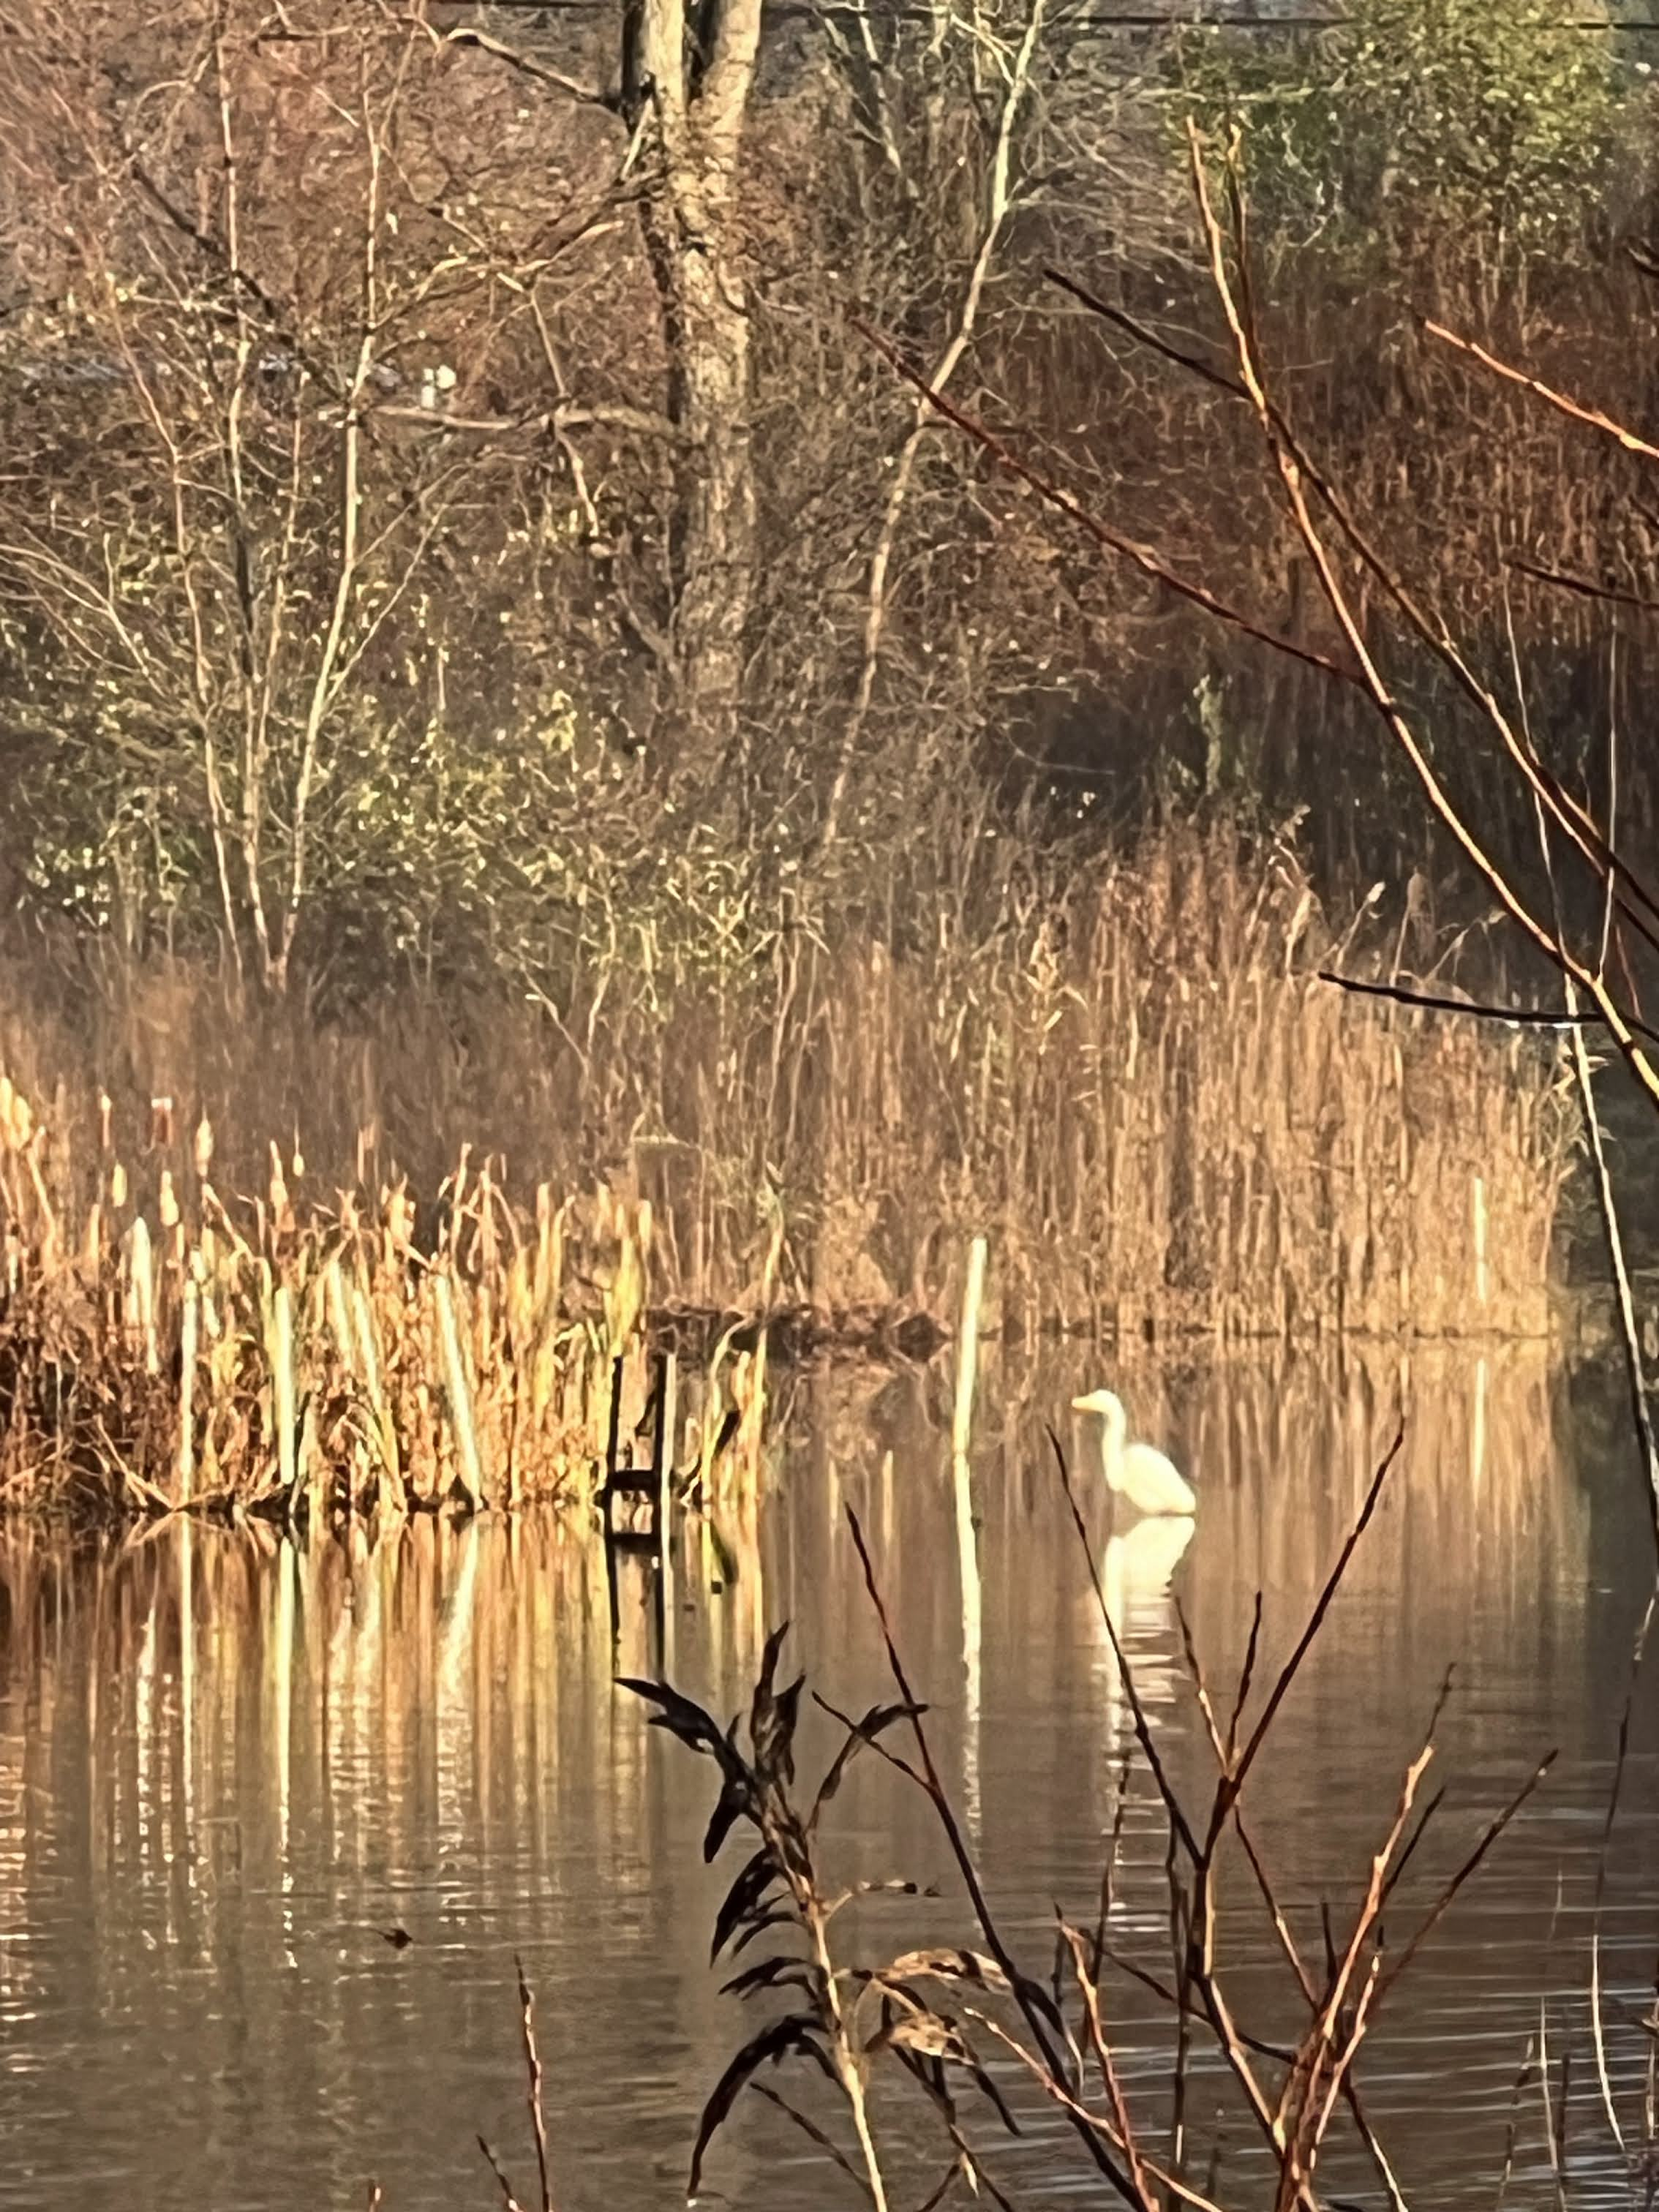
\includegraphics[scale=.1]{Research/HANA/NOV2024/IMG_9800.JPG}
\caption{HANA Tree Study}
\label{fig:HANA}
\end{figure}

\begin{figure}[h!]
\centering
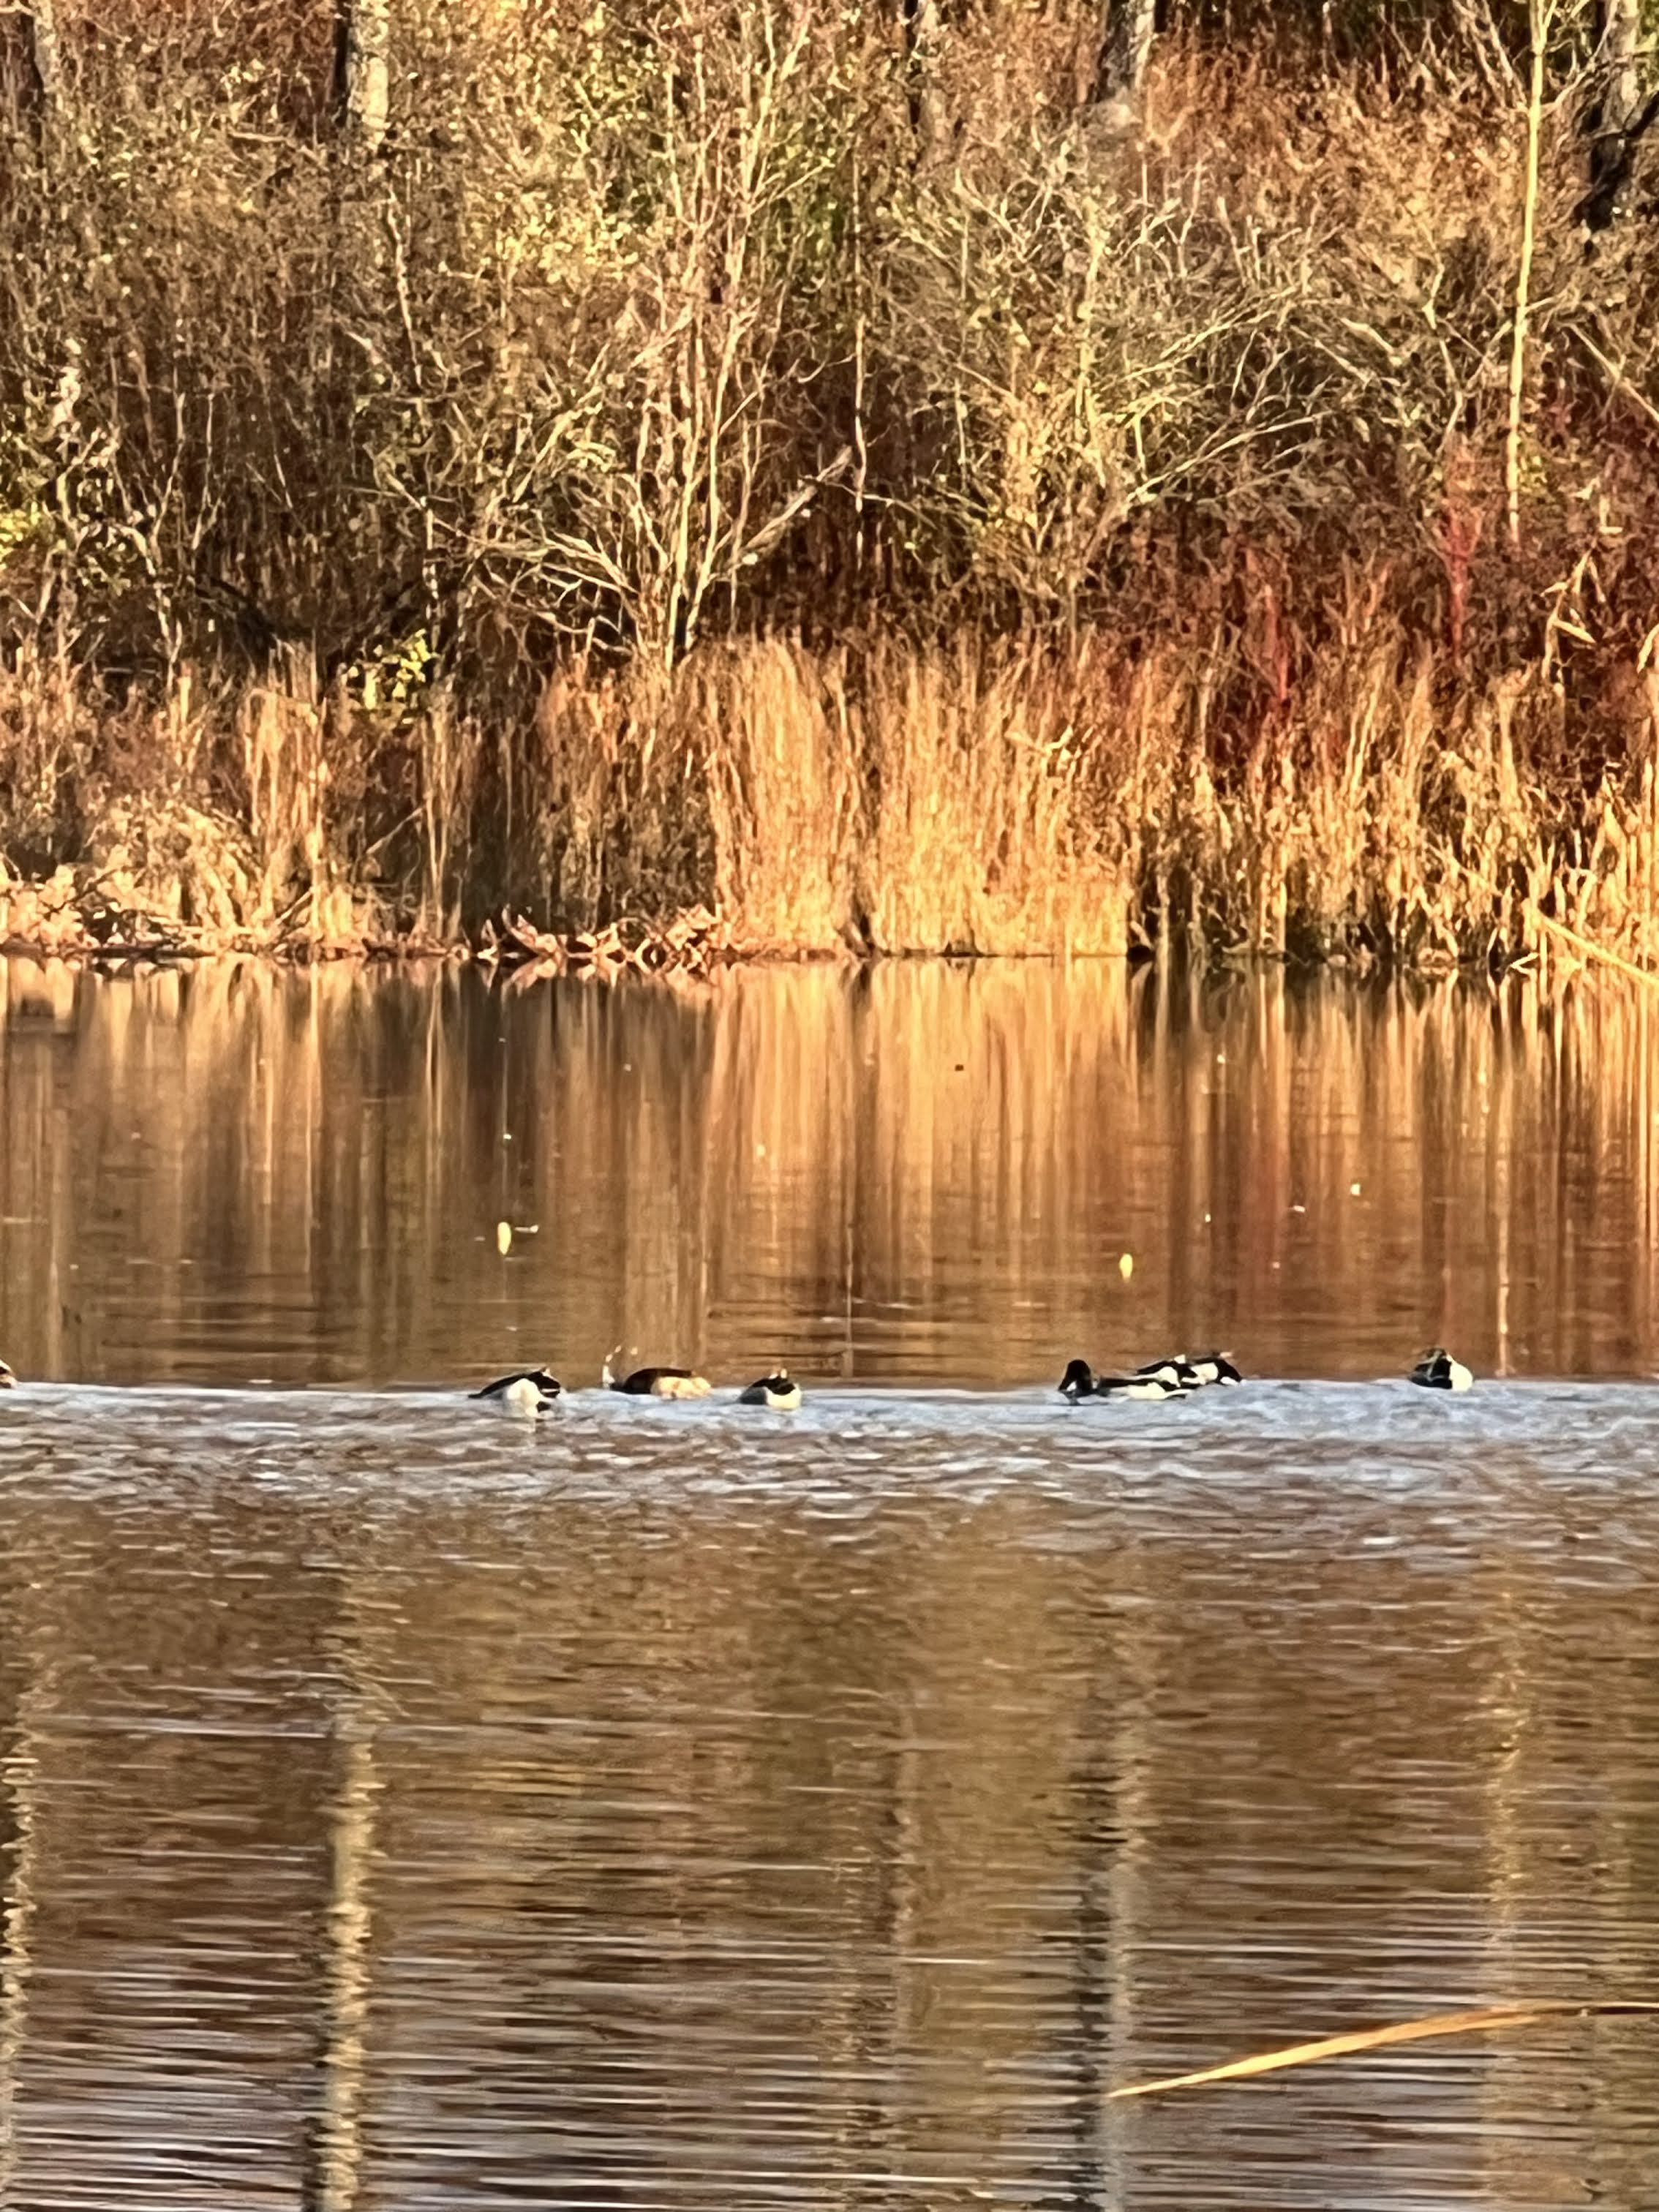
\includegraphics[scale=.1]{Research/HANA/NOV2024/IMG_9811.JPG}
\caption{HANA Tree Study}
\label{fig:HANA}
\end{figure}

\begin{figure}[h!]
\centering
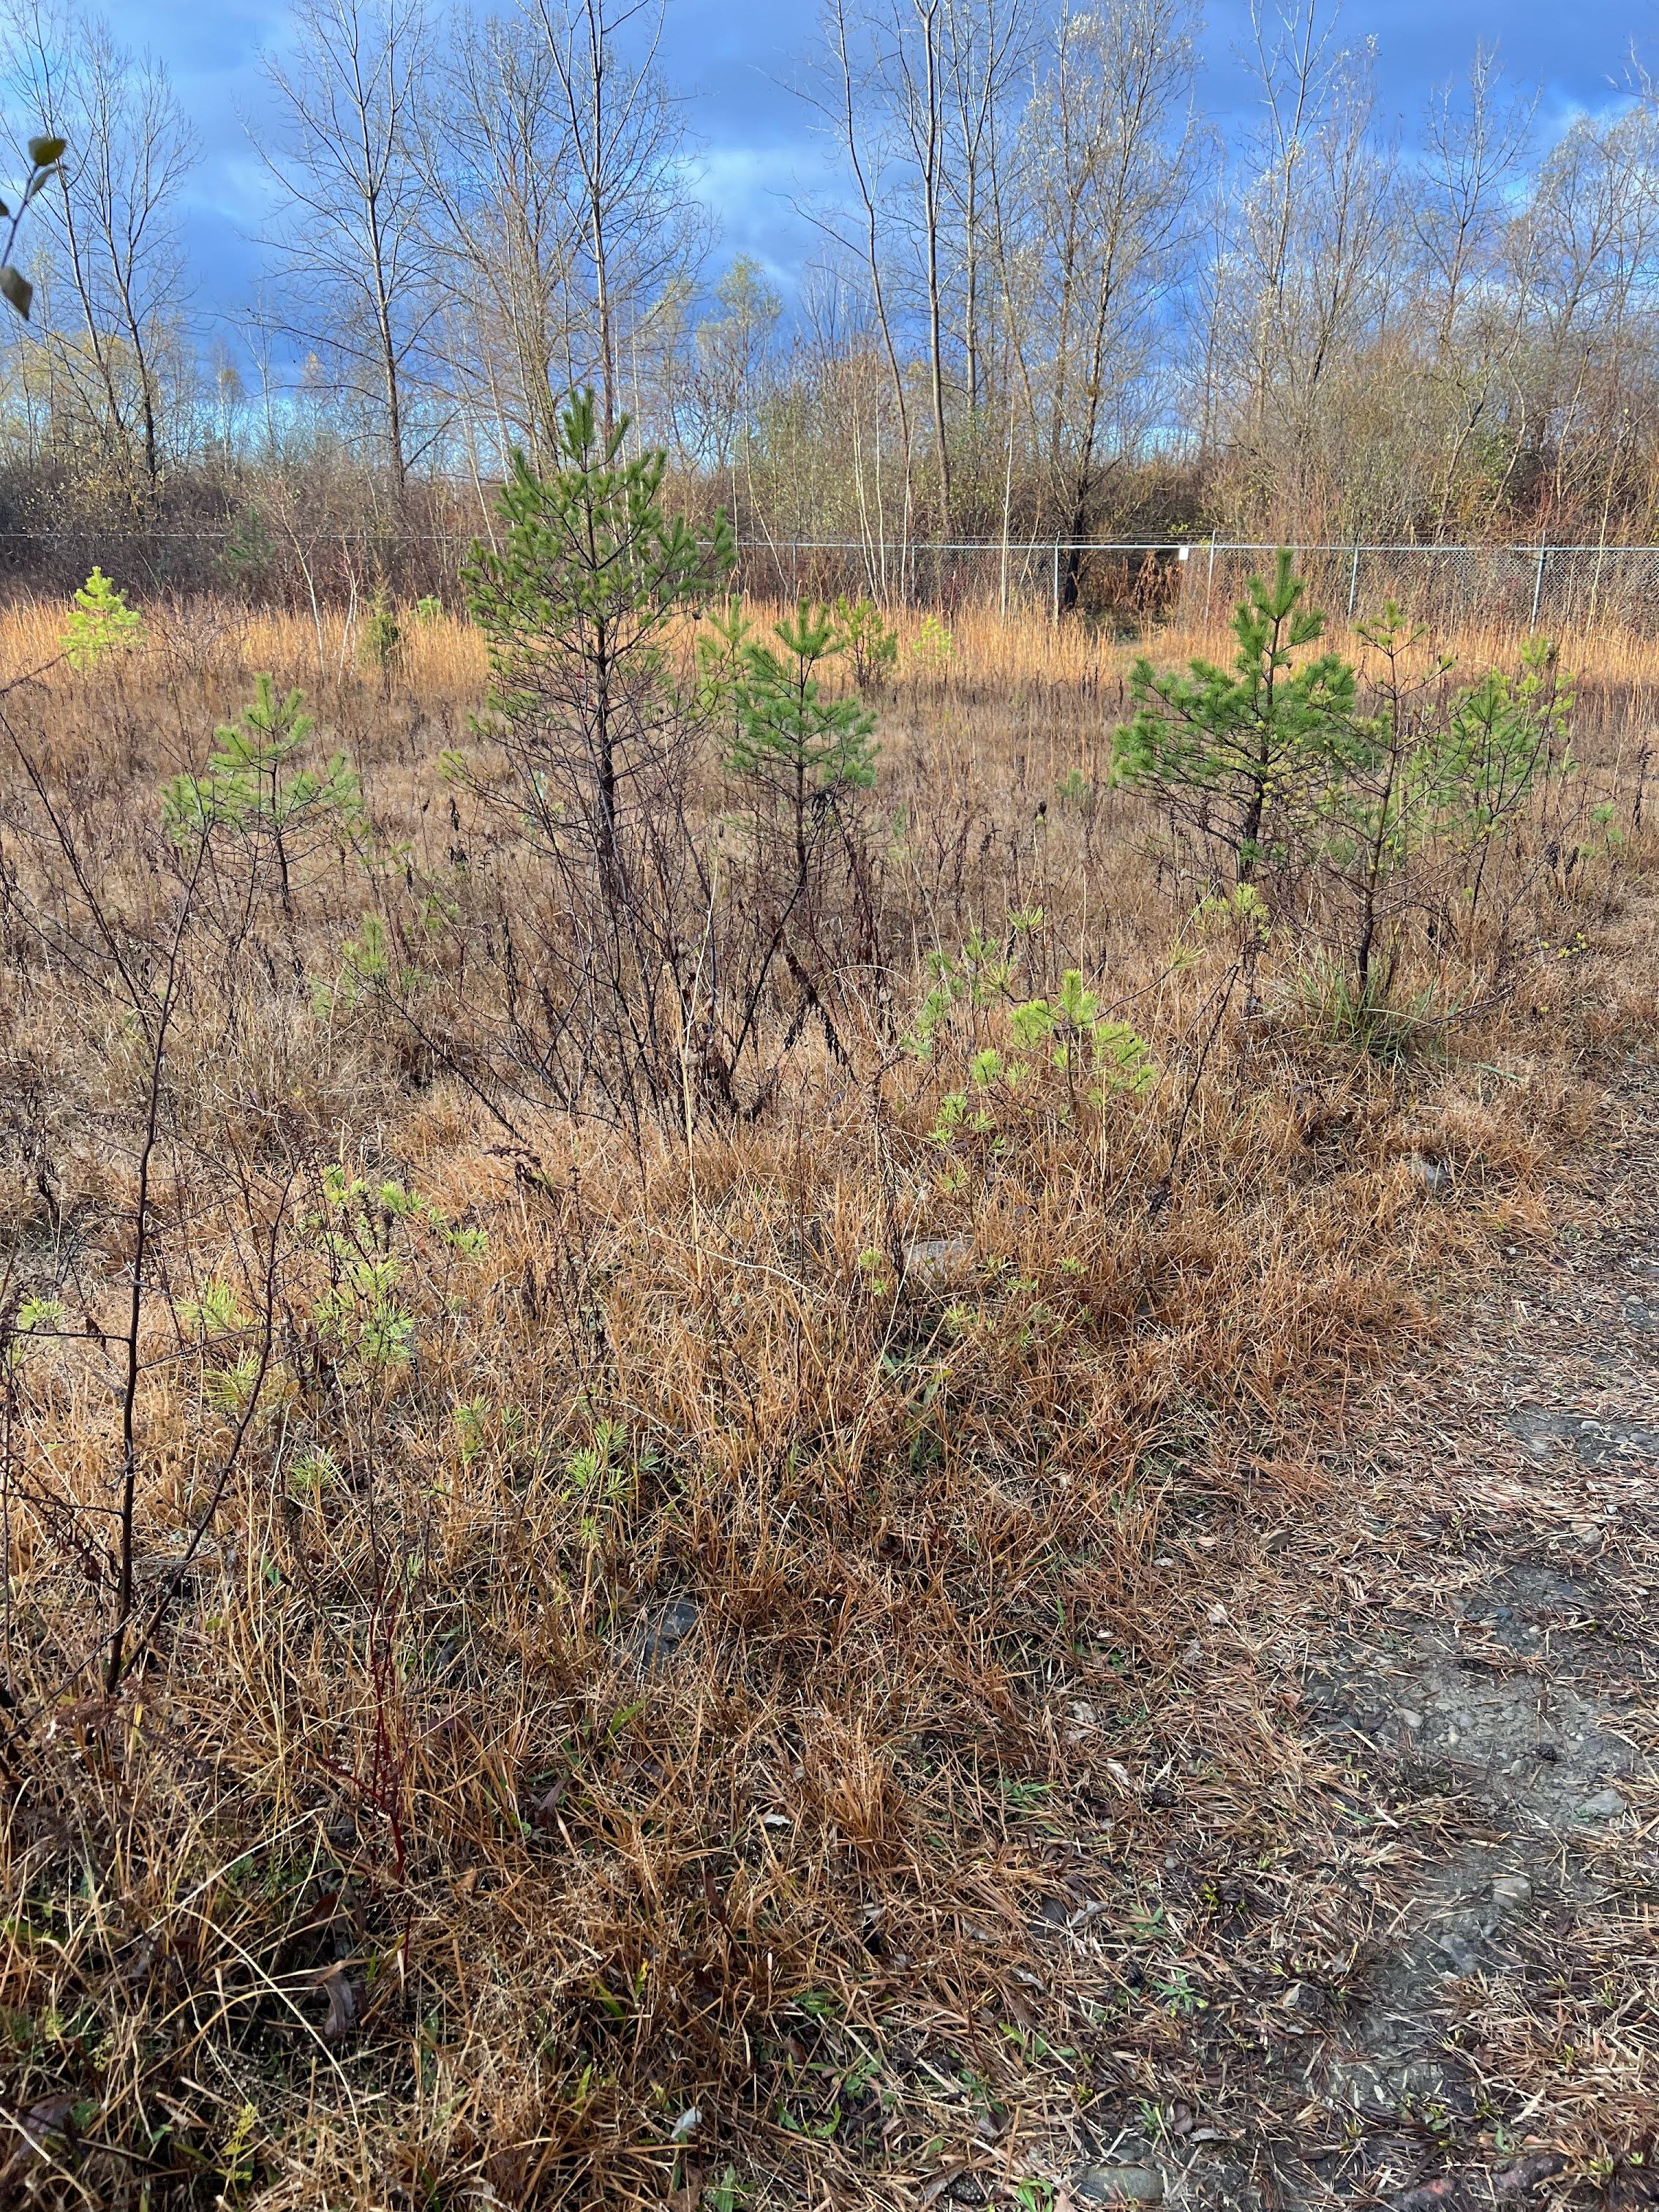
\includegraphics[scale=.1]{Research/HANA/NOV2024/IMG_9820.JPG}
\caption{HANA Tree Study}
\label{fig:HANA}
\end{figure}

\begin{figure}[h!]
\centering
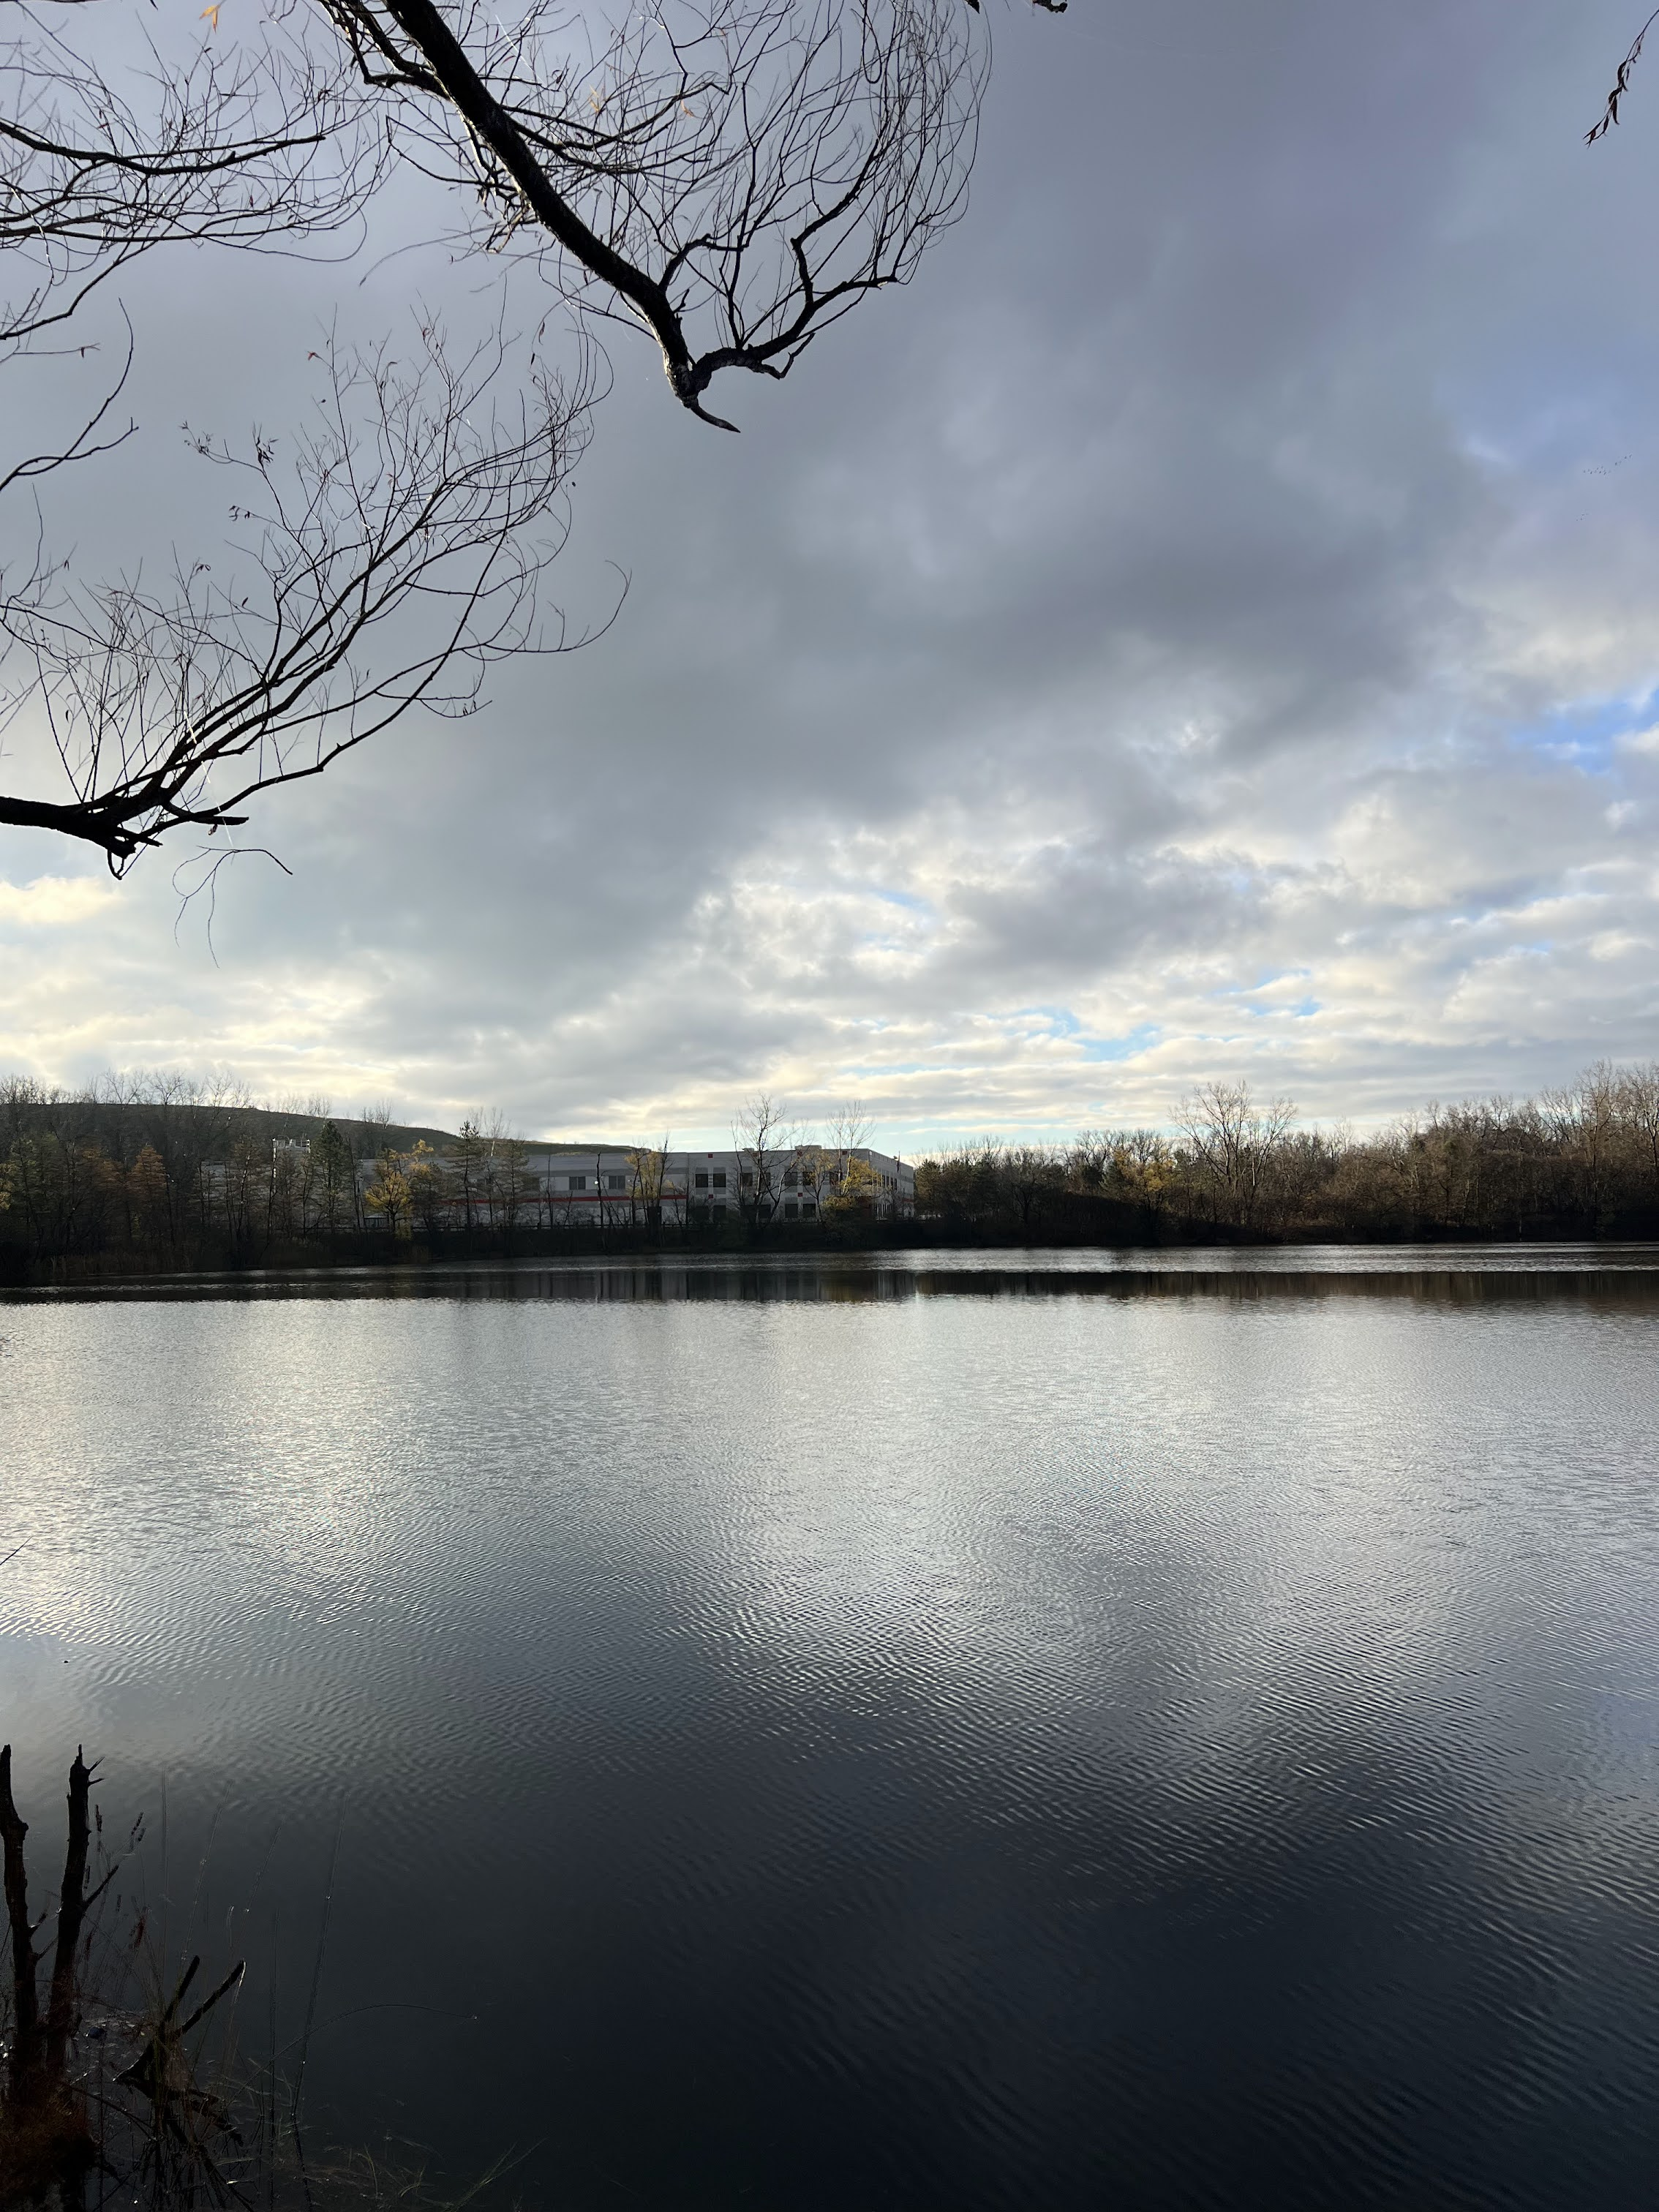
\includegraphics[scale=.1]{Research/HANA/NOV2024/IMG_9830.JPG}
\caption{HANA Tree Study}
\label{fig:HANA}
\end{figure}

\begin{figure}[h!]
\centering
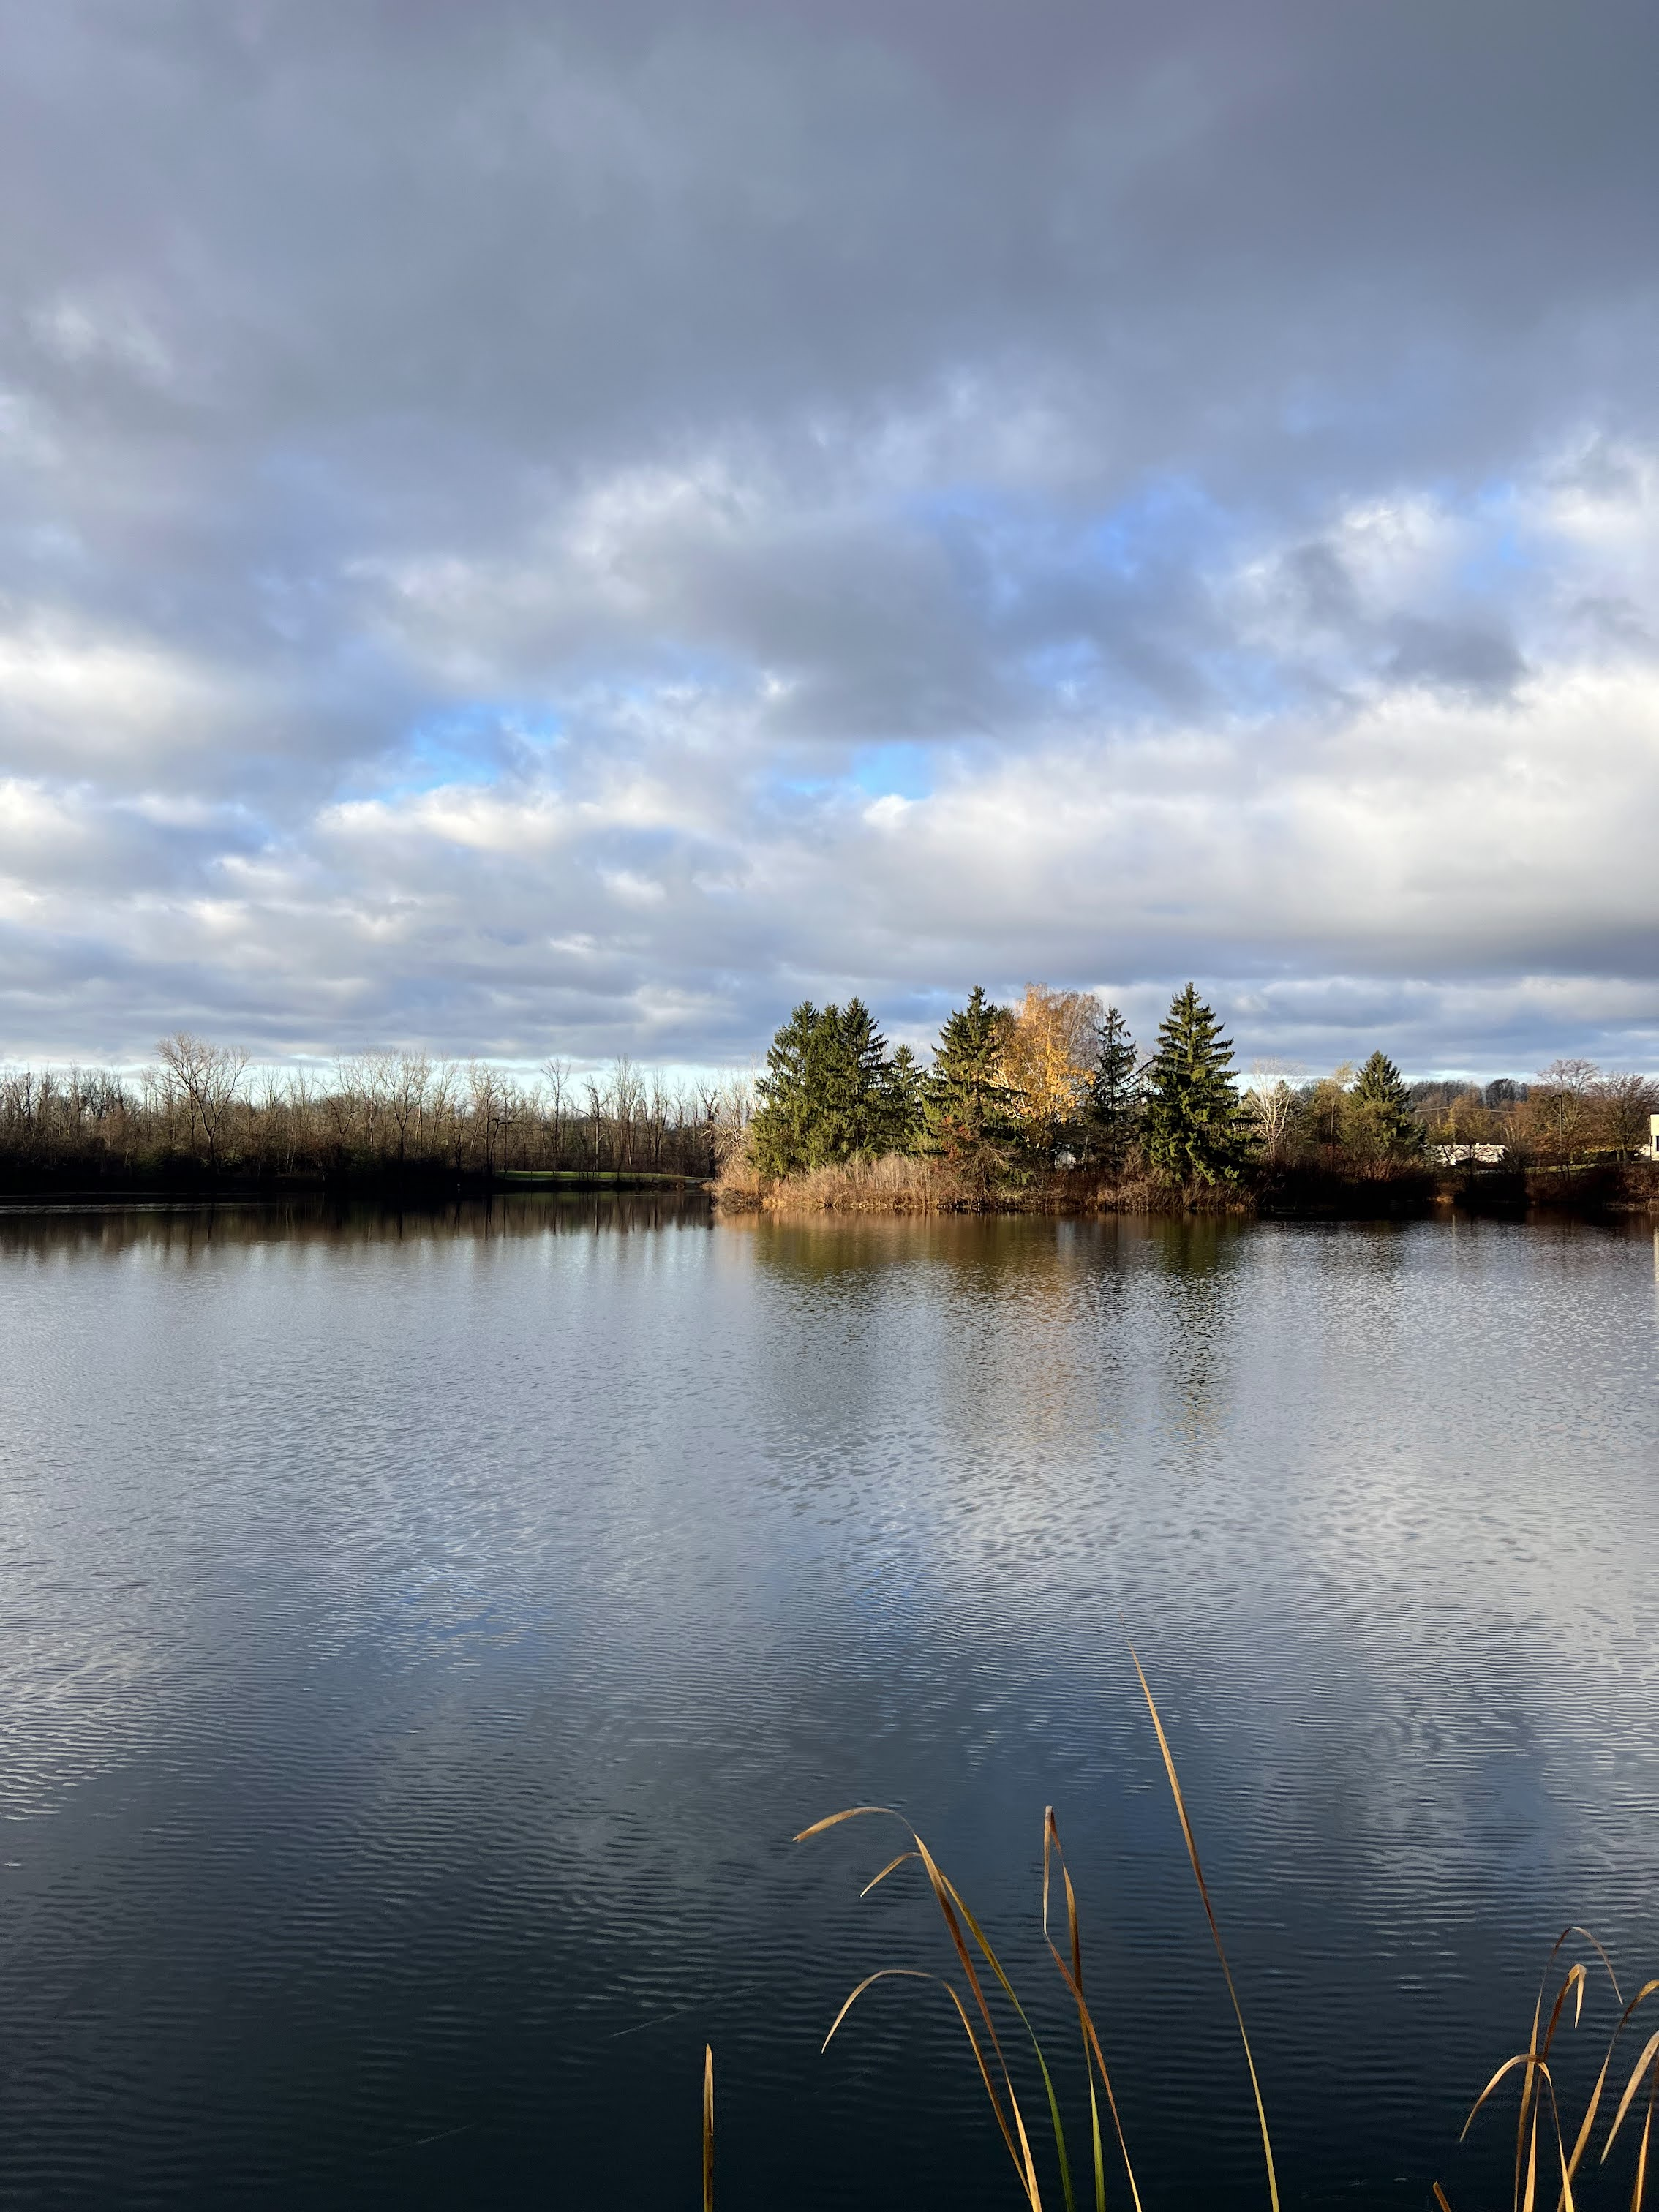
\includegraphics[scale=.1]{Research/HANA/NOV2024/IMG_9834.JPG}
\caption{HANA Tree Study}
\label{fig:HANA}
\end{figure}

\begin{figure}[h!]
\centering
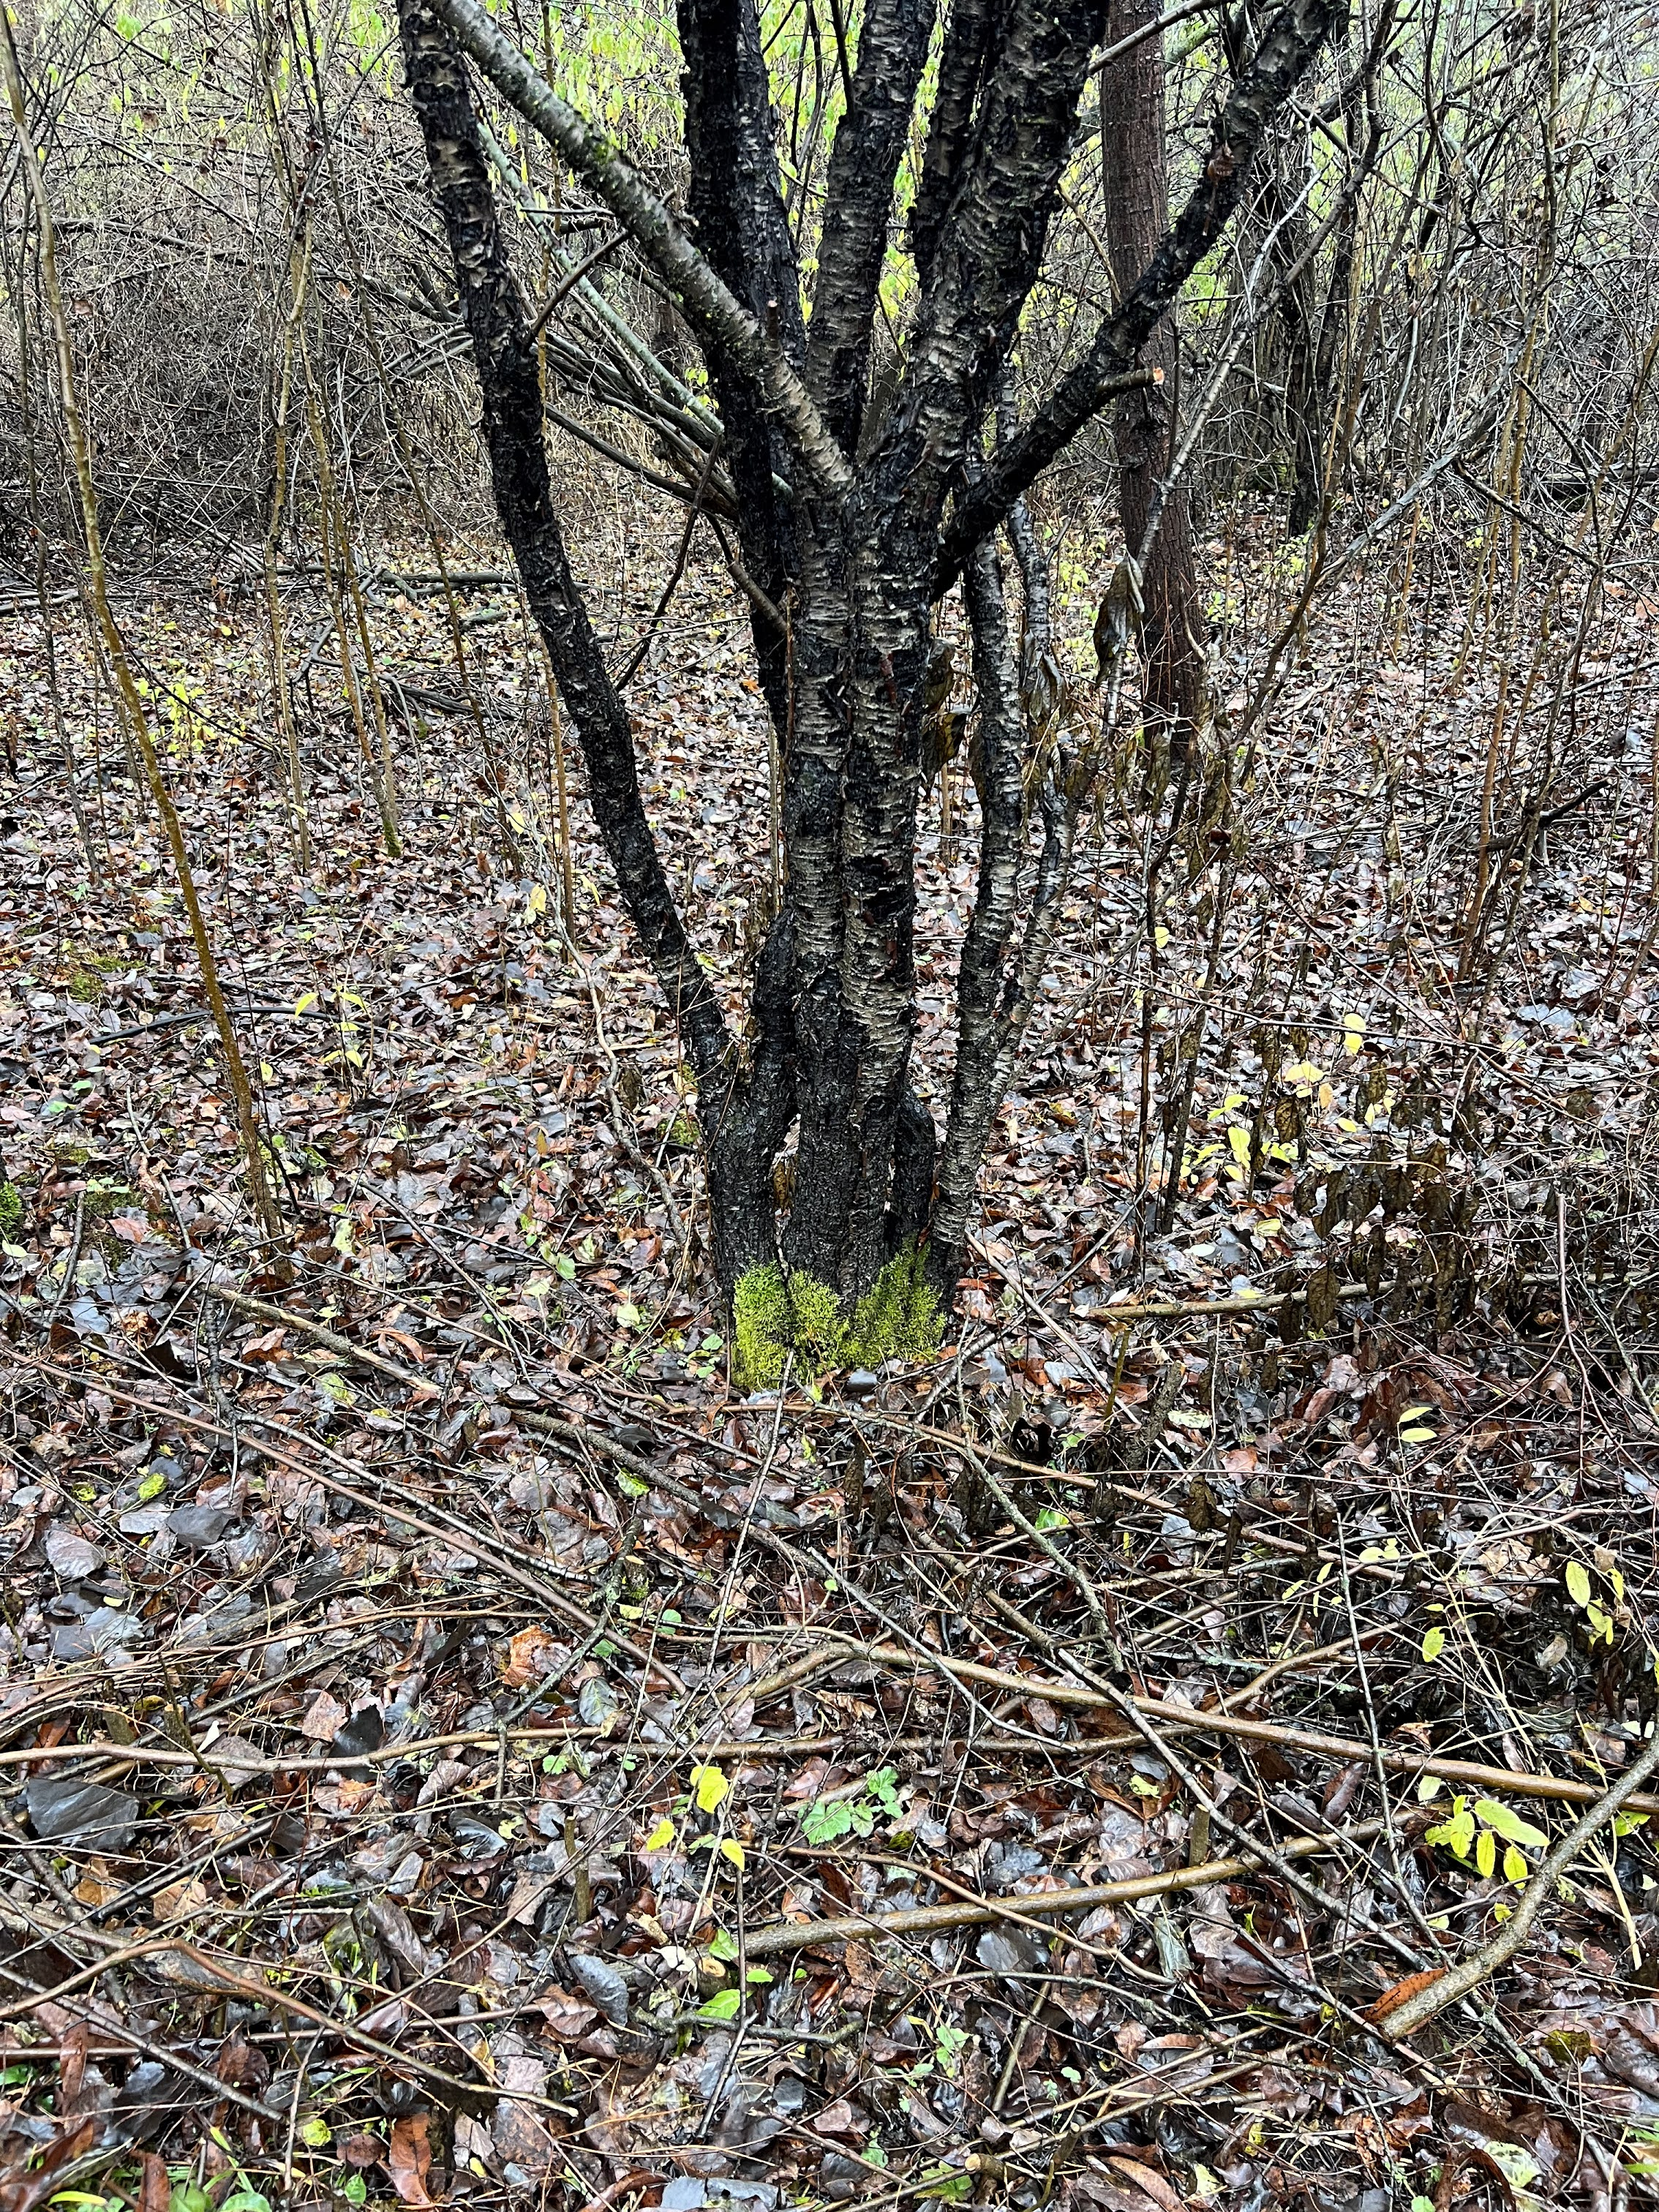
\includegraphics[scale=.1]{Research/HANA/NOV2024/IMG_9845.JPG}
\caption{HANA Tree Study}
\label{fig:HANA}
\end{figure}



\begin{figure}[h!]
\centering
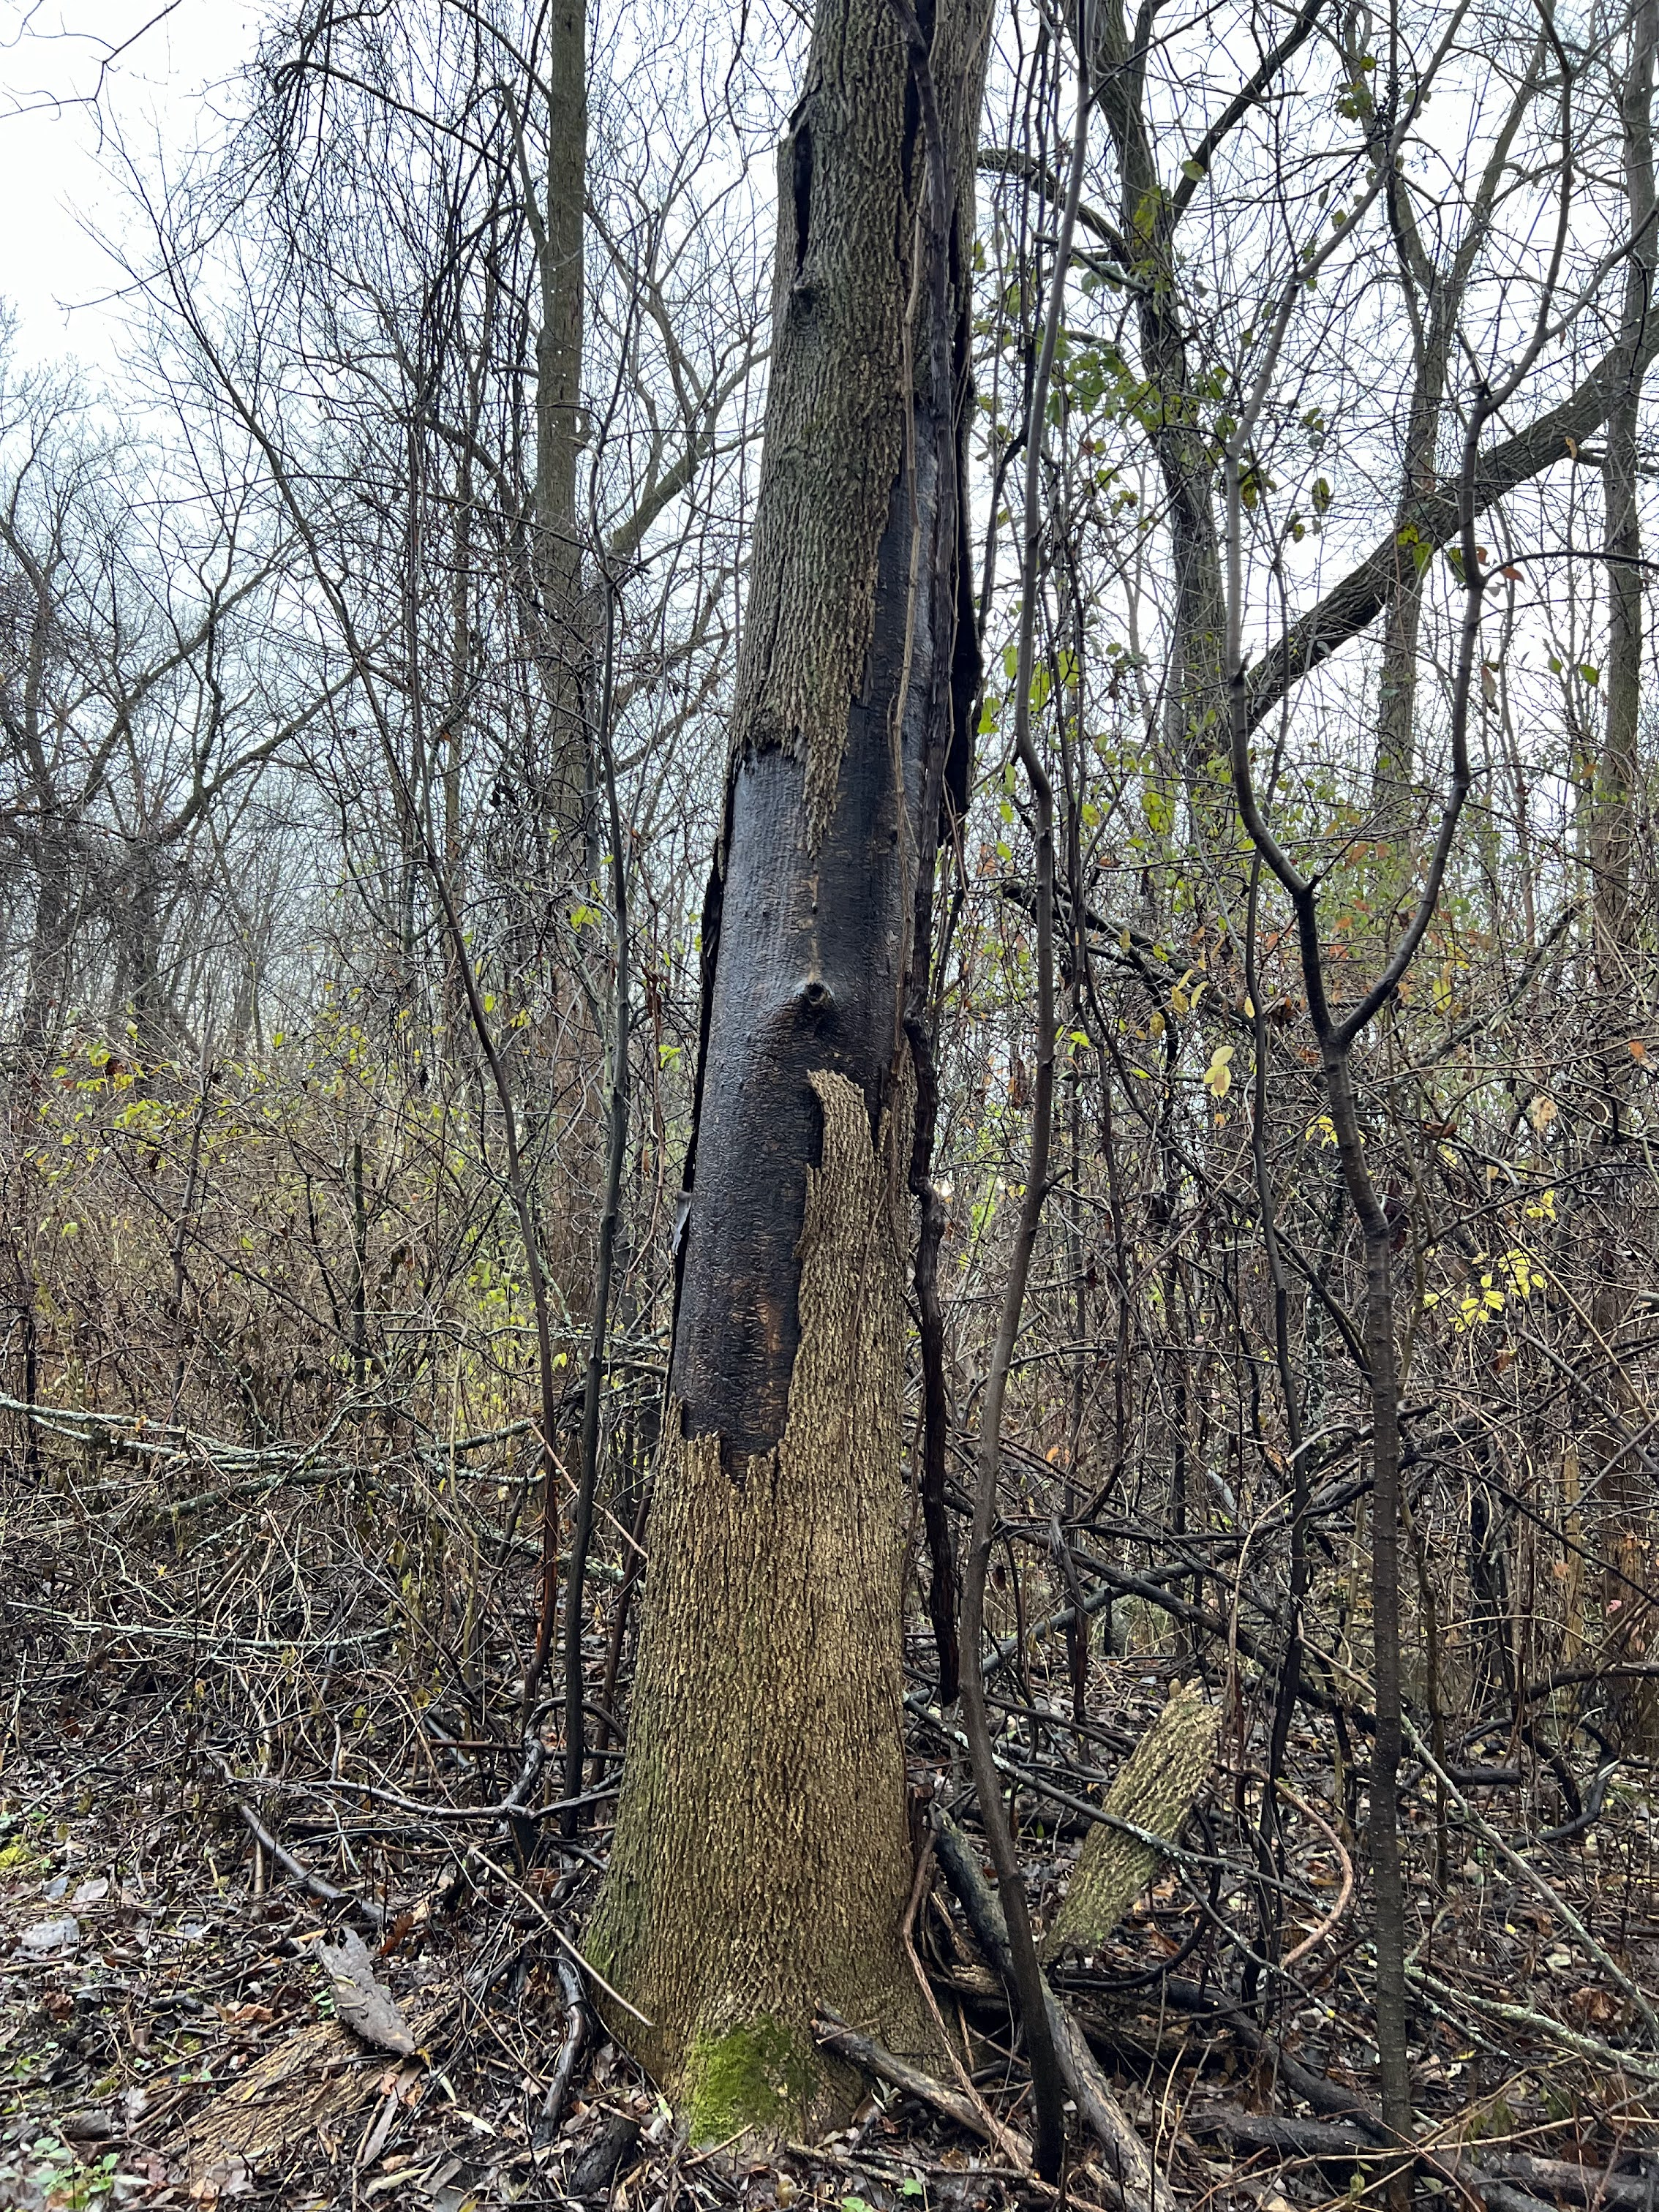
\includegraphics[scale=.1]{Research/HANA/NOV2024/IMG_9848.JPG}
\caption{HANA Tree Study}
\label{fig:HANA}
\end{figure}


\begin{figure}[h!]
\centering
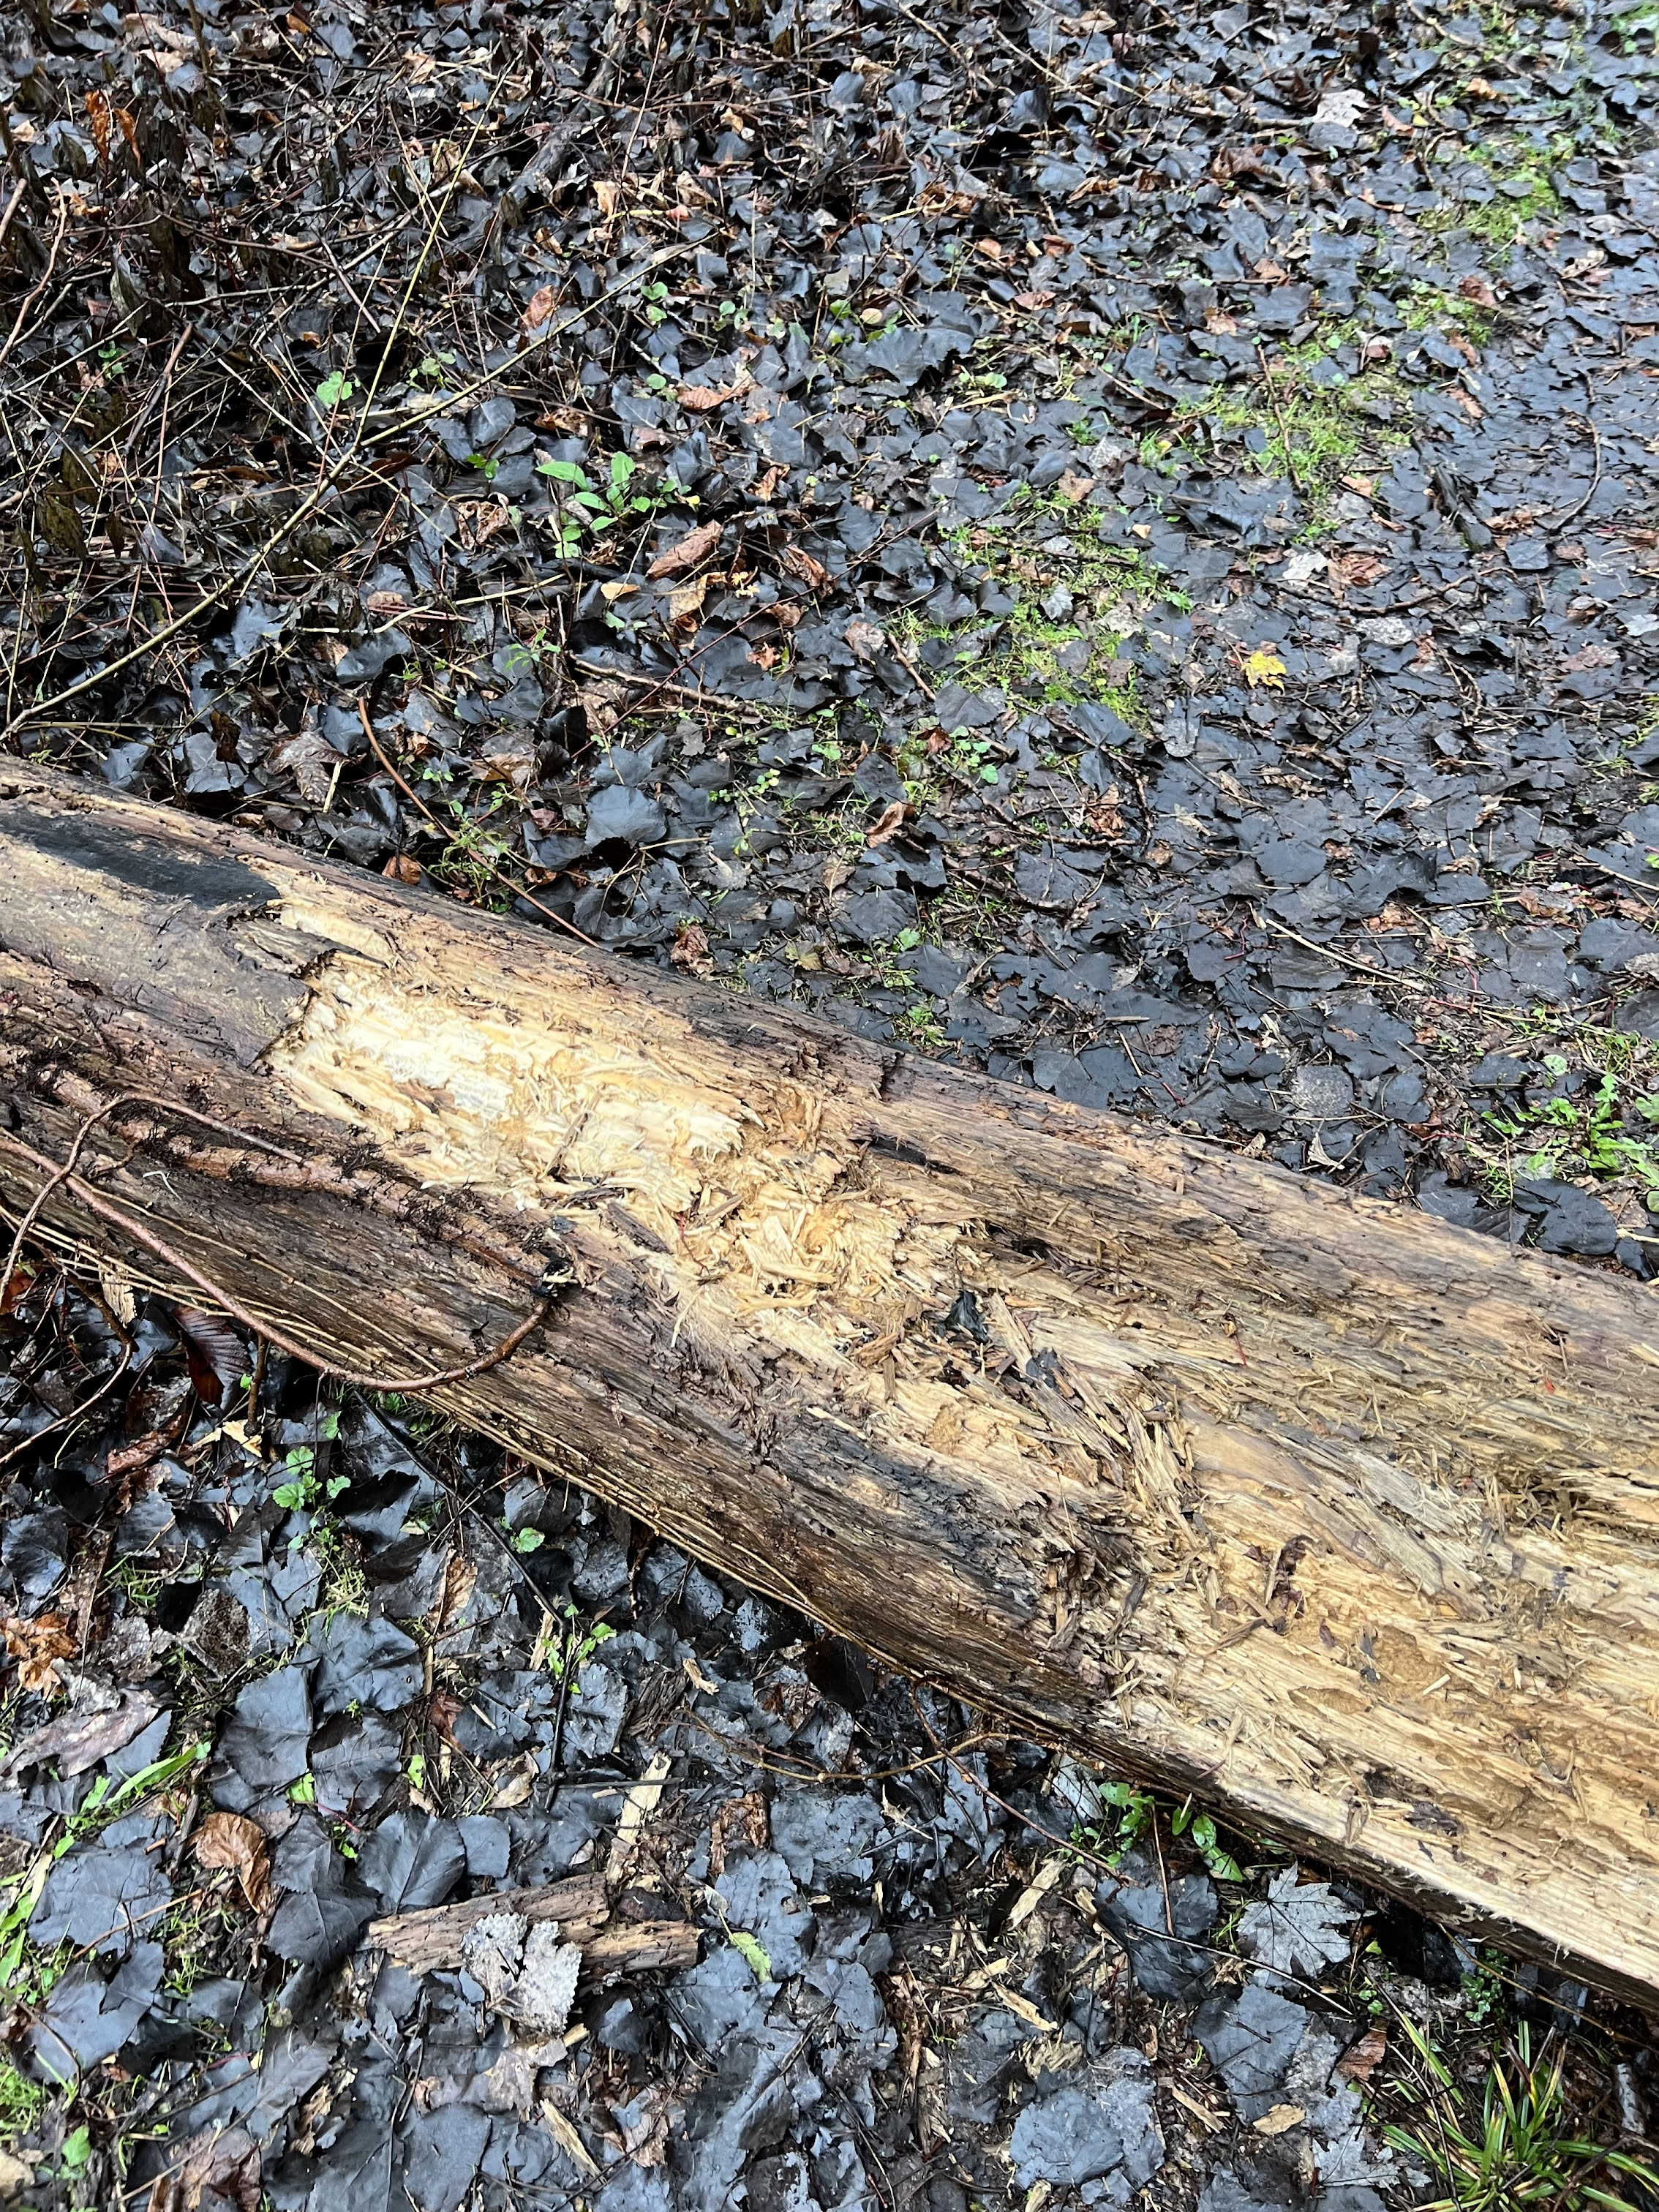
\includegraphics[scale=.1]{Research/HANA/NOV2024/IMG_9852.JPG}
\caption{HANA Tree Study}
\label{fig:HANA}
\end{figure}



\begin{figure}[h!]
\centering
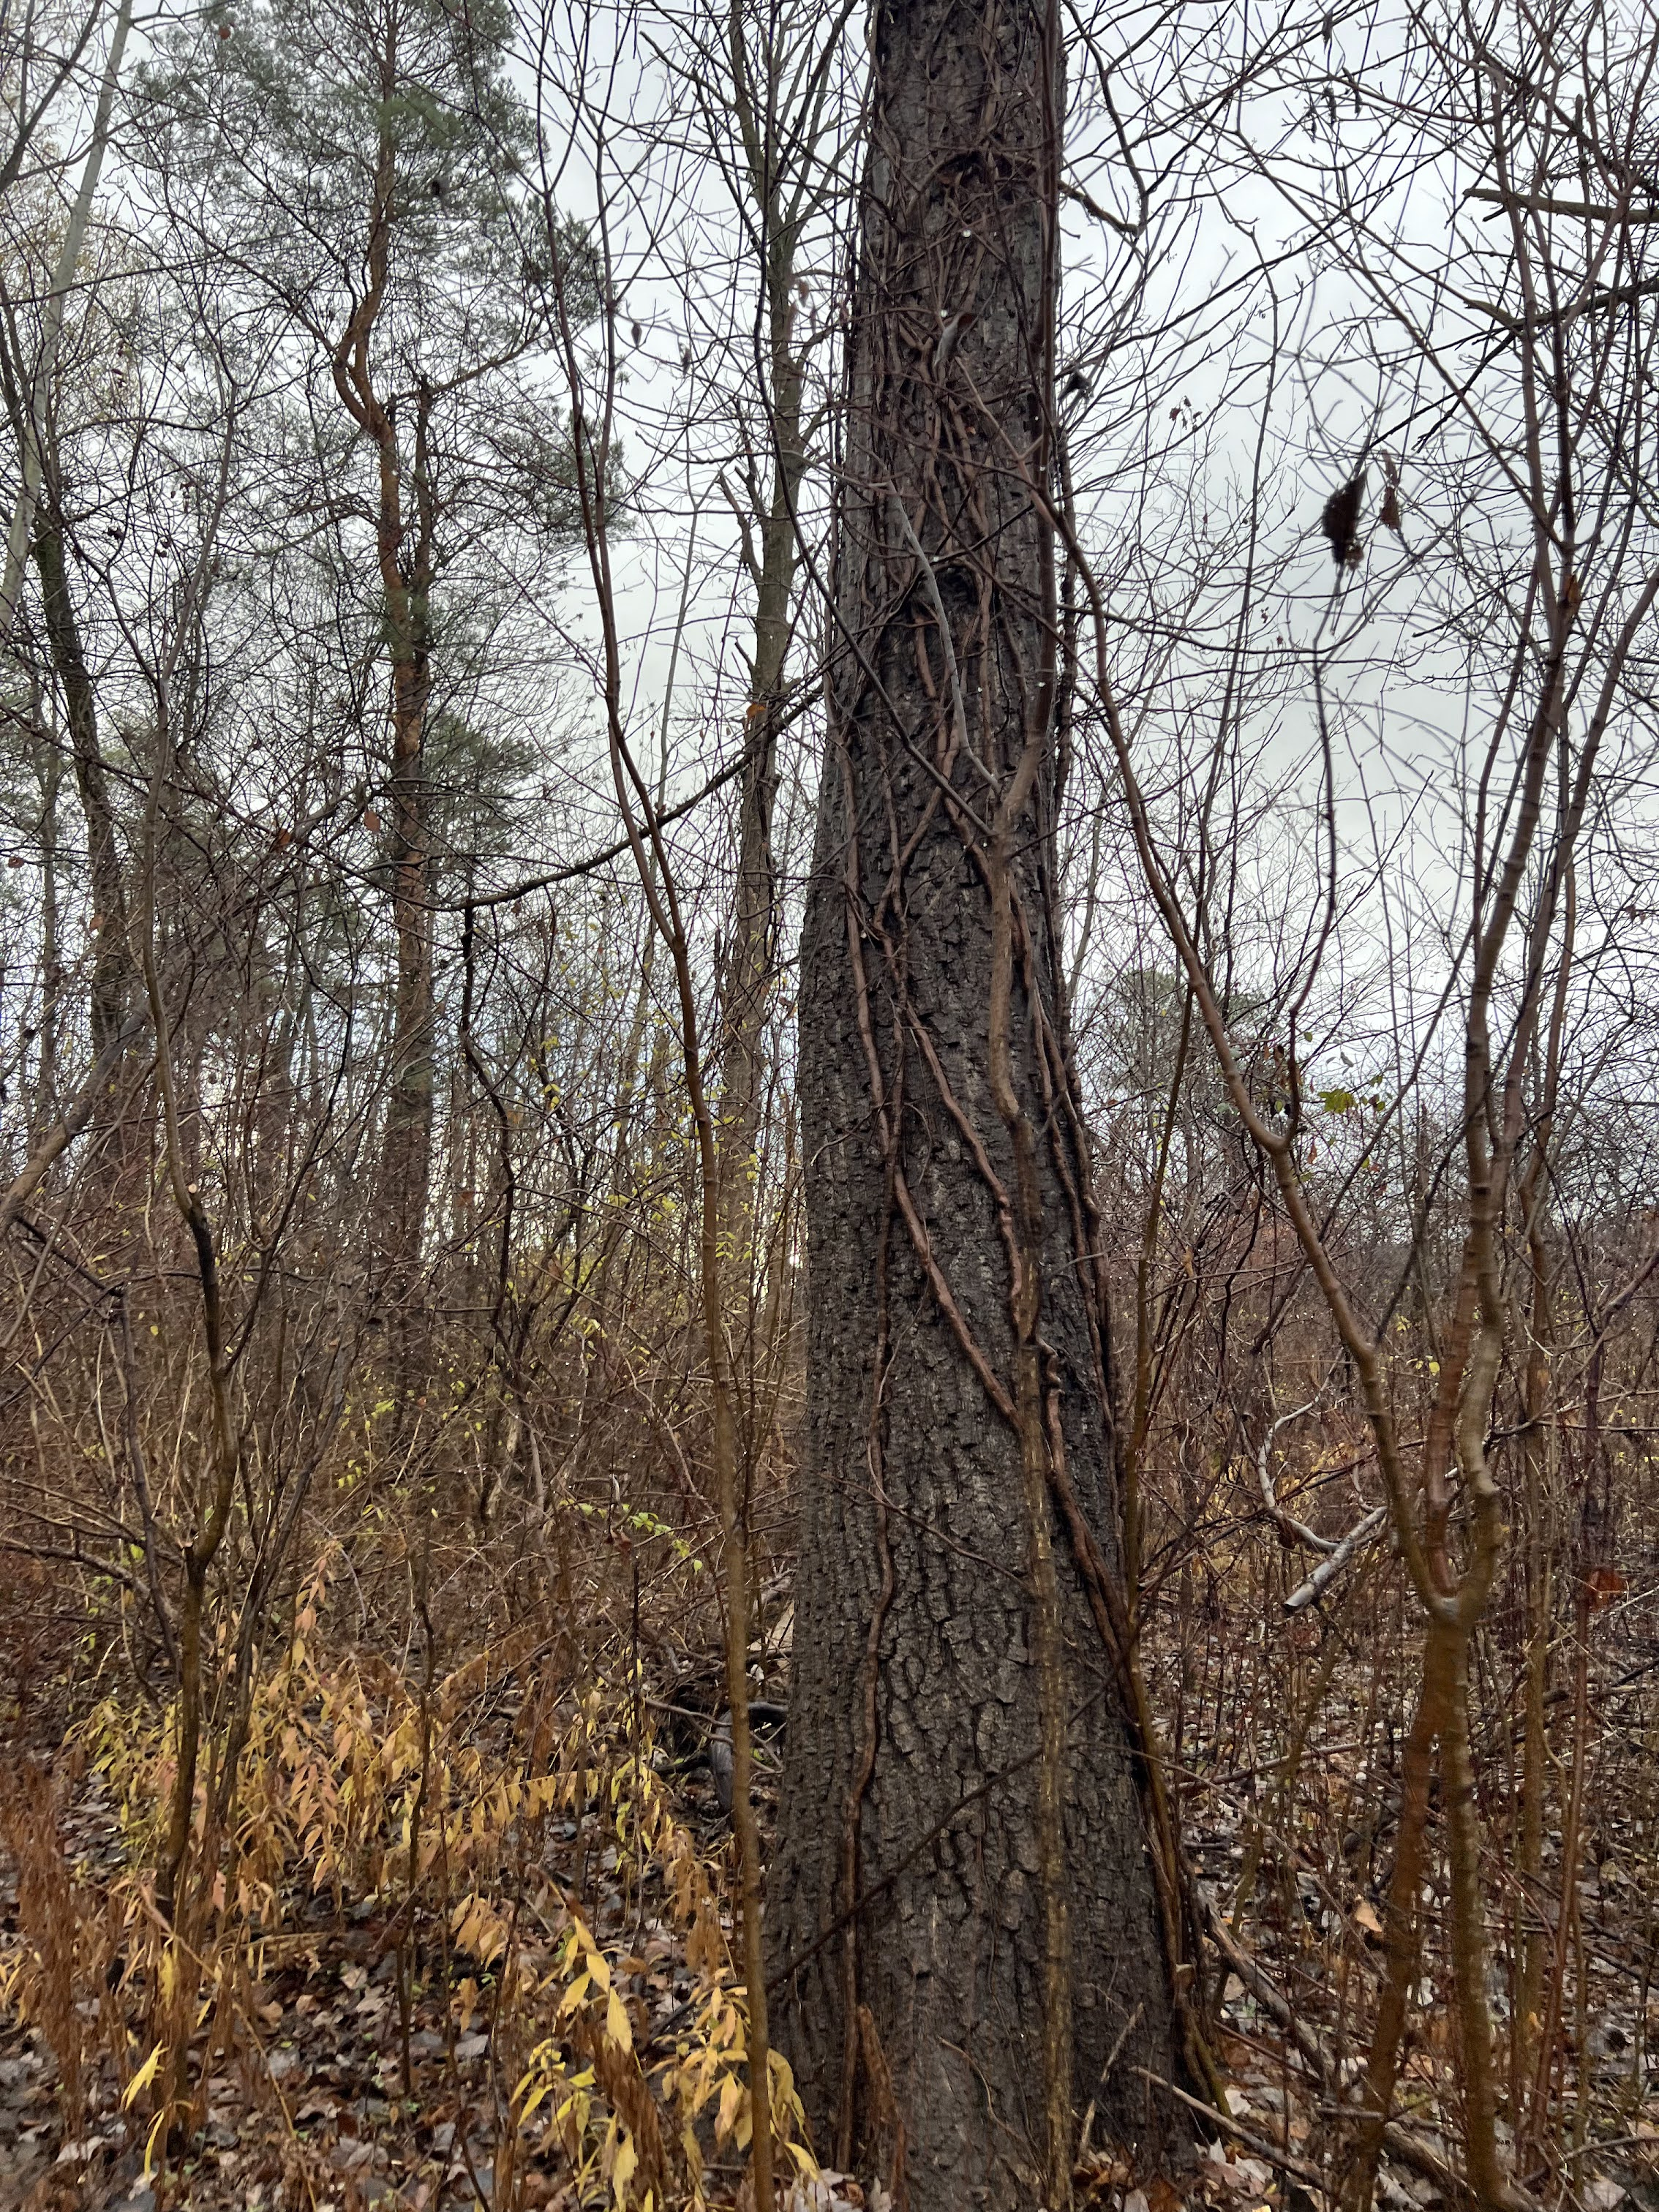
\includegraphics[scale=.1]{Research/HANA/NOV2024/IMG_9856.JPG}
\caption{HANA Tree Study}
\label{fig:HANA}
\end{figure}


\begin{figure}[h!]
\centering
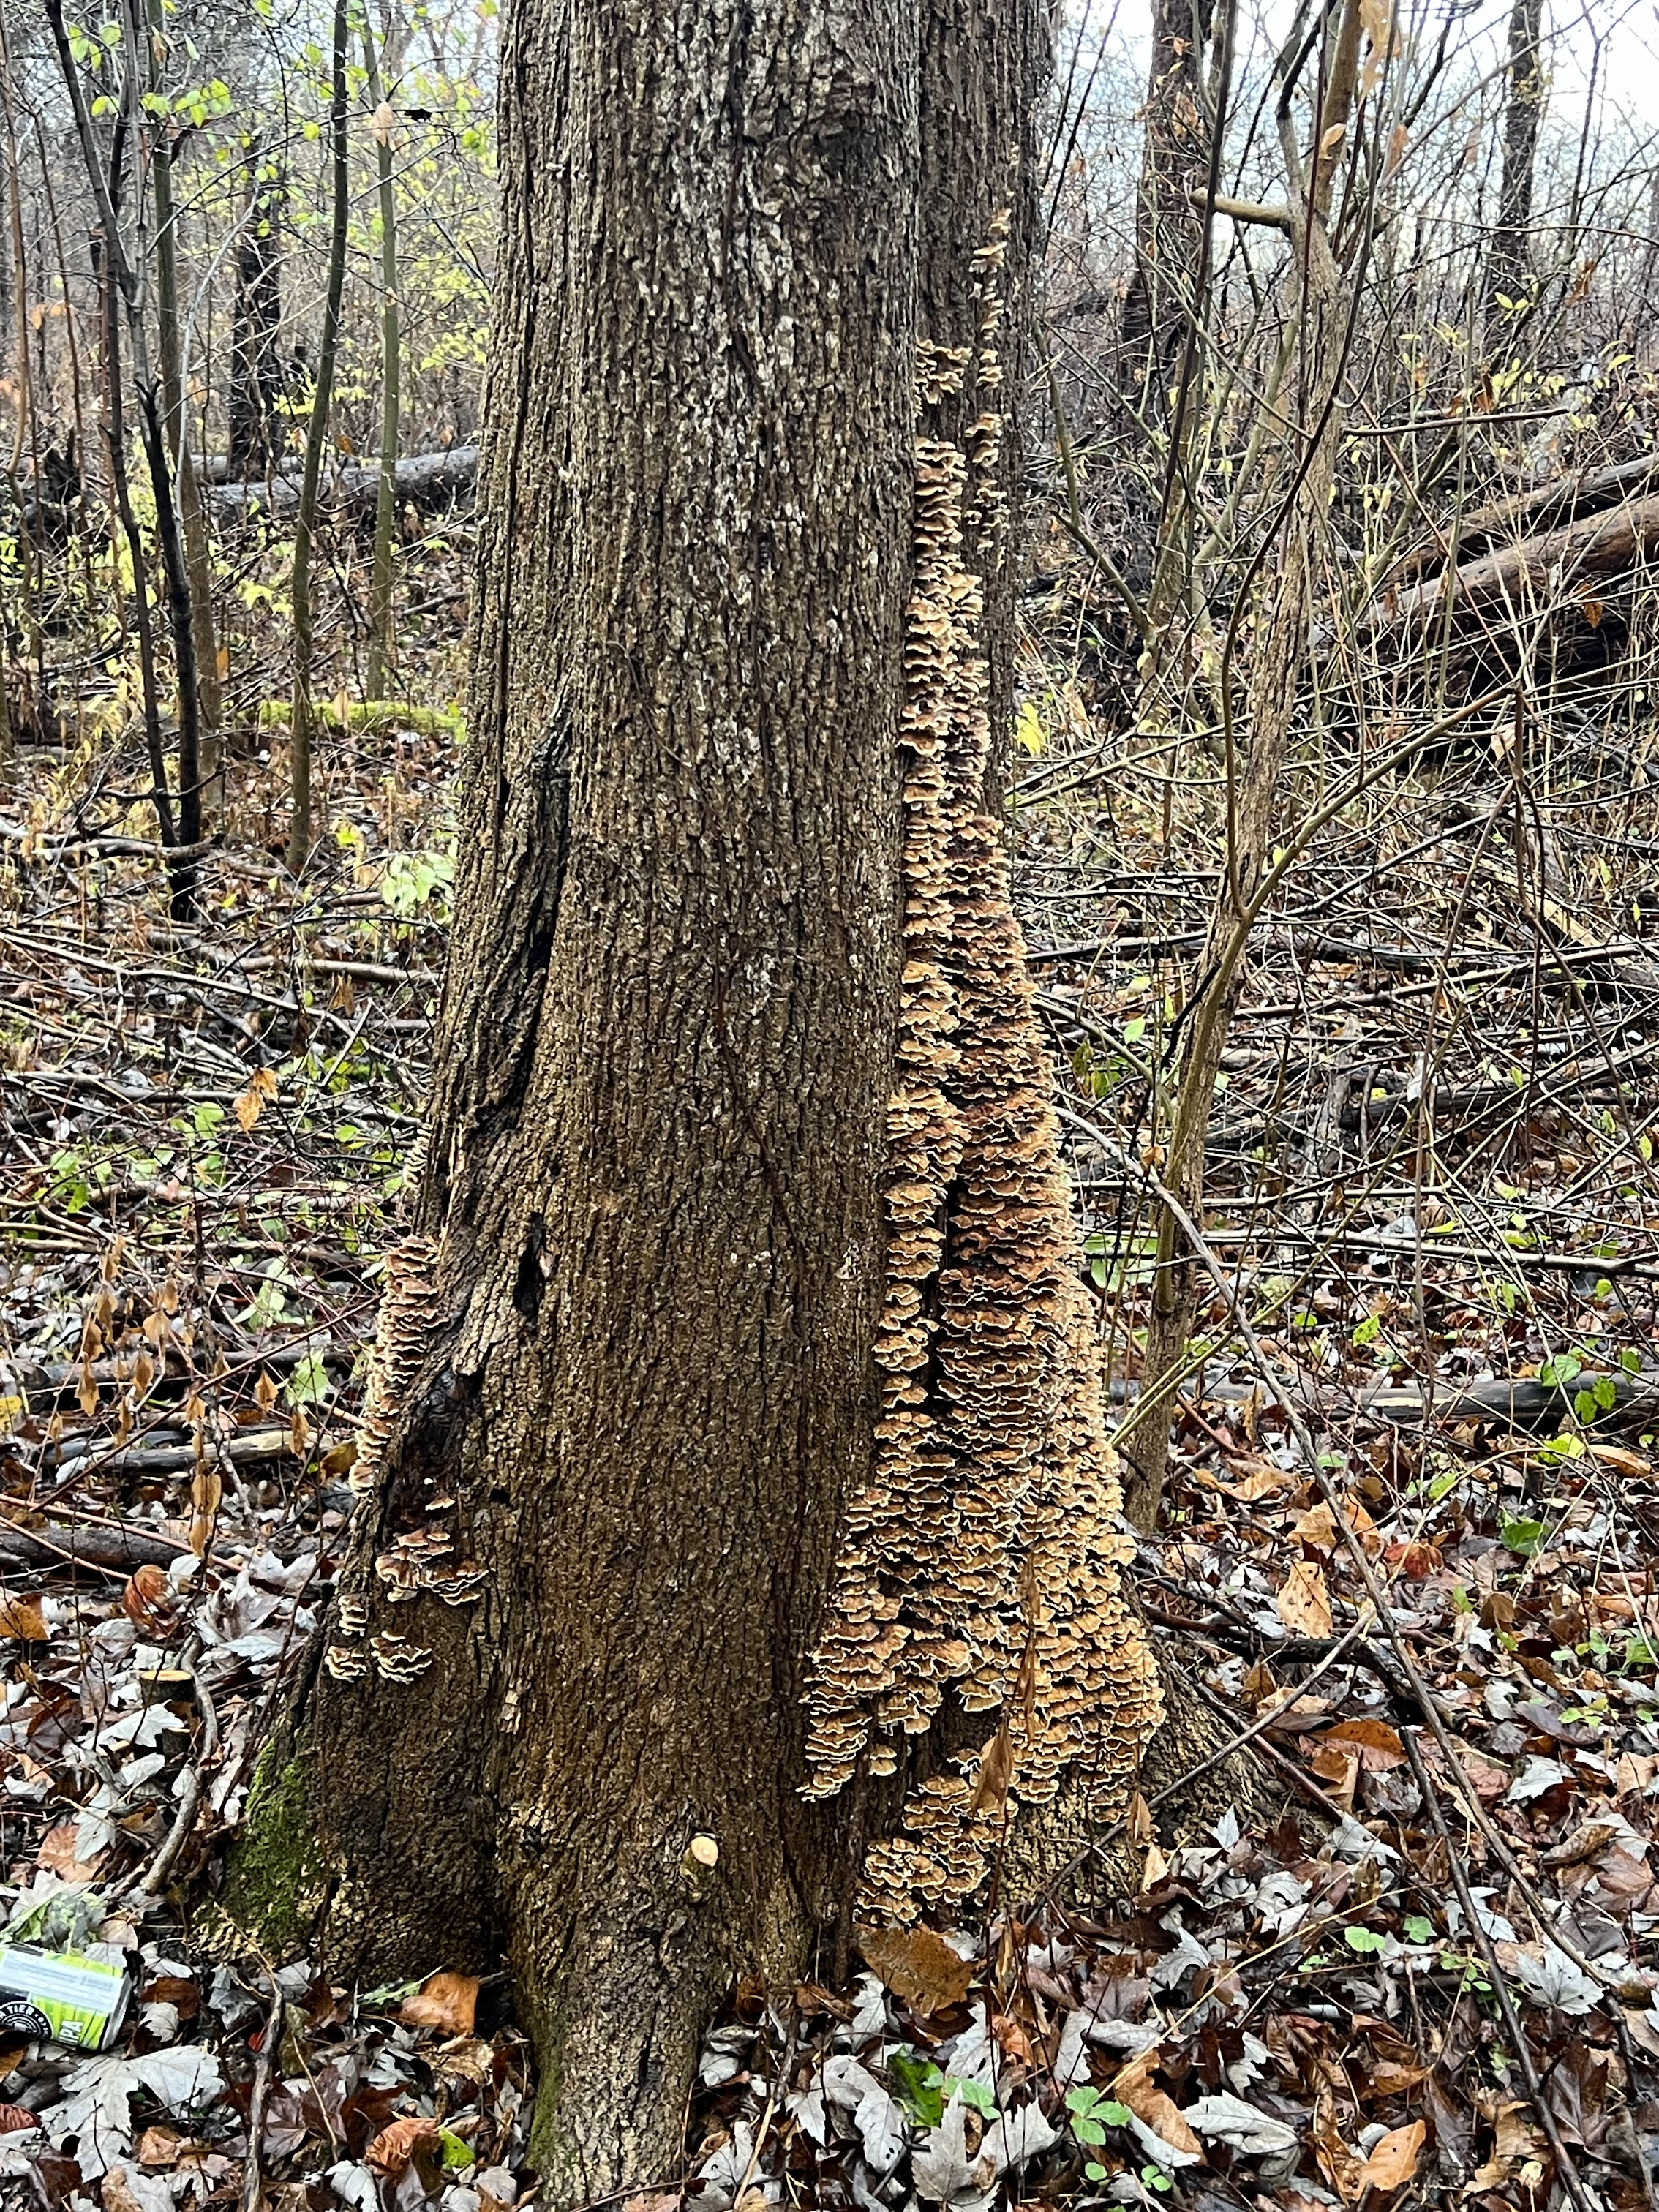
\includegraphics[scale=.1]{Research/HANA/NOV2024/IMG_9859.JPG}
\caption{HANA Tree Study}
\label{fig:HANA}
\end{figure}


\begin{figure}[h!]
\centering
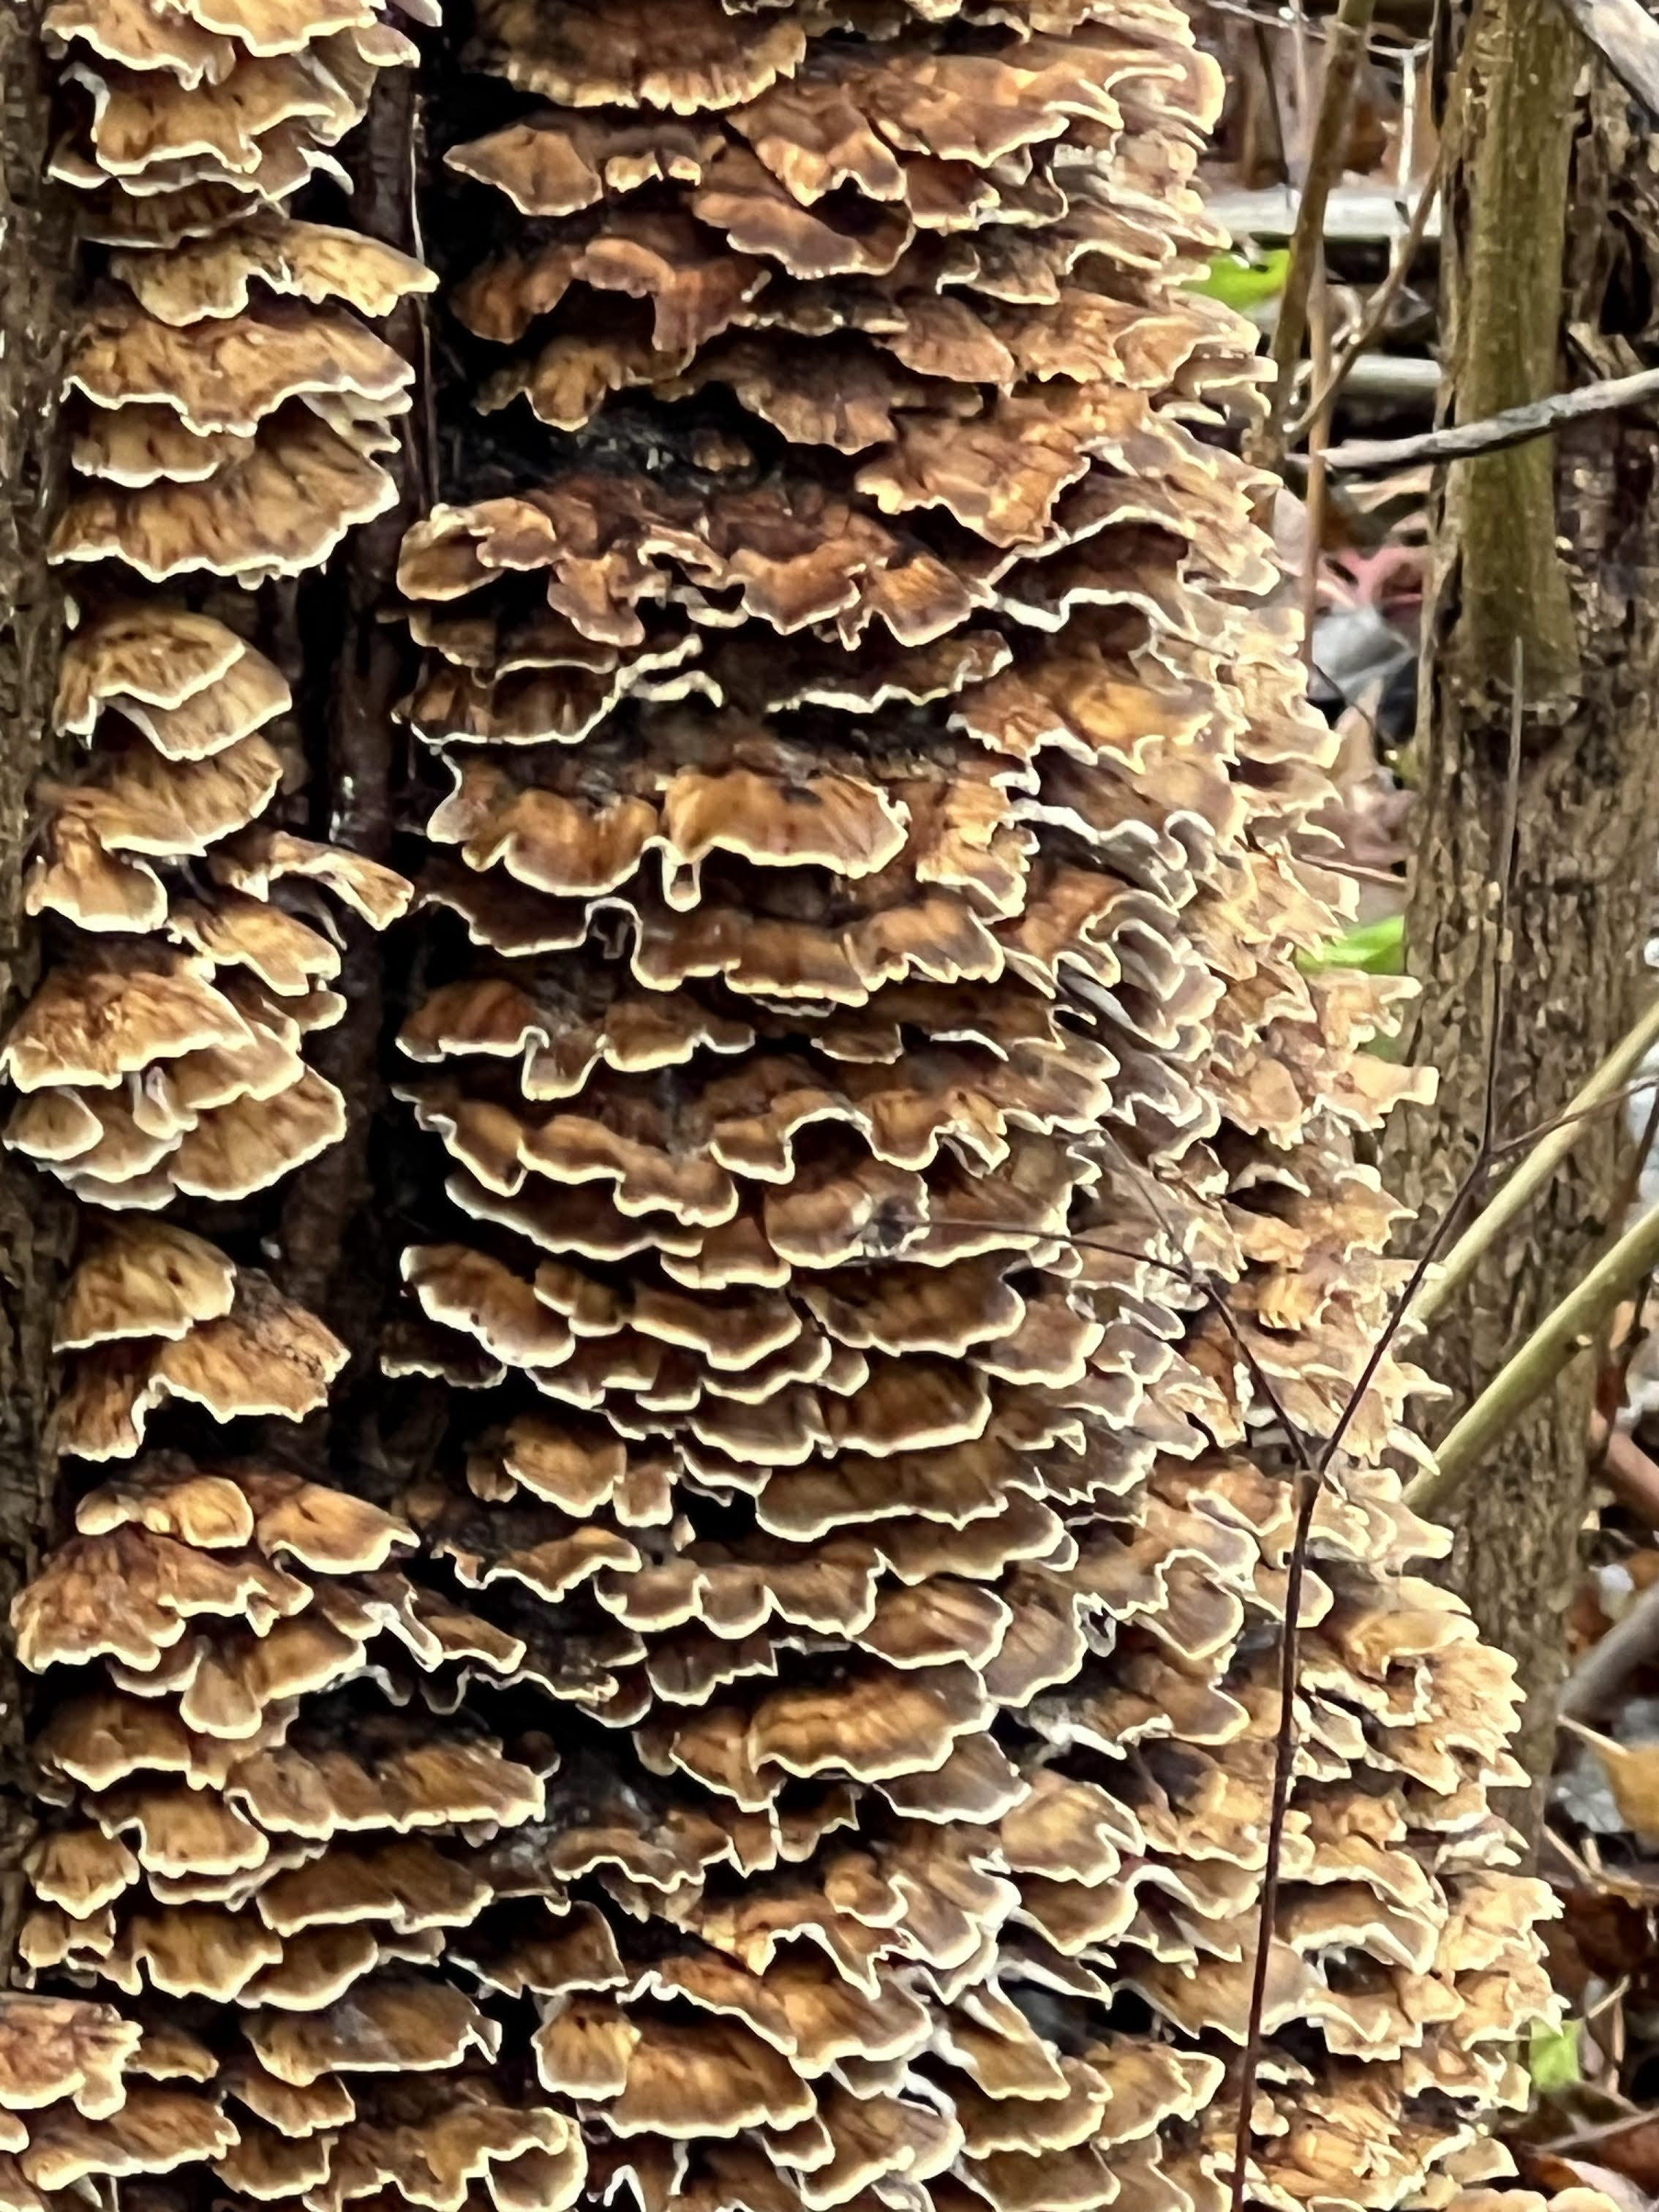
\includegraphics[scale=.1]{Research/HANA/NOV2024/IMG_9860.JPG}
\caption{HANA Tree Study}
\label{fig:HANA}
\end{figure}


\clearpage
\section{Bibliography}
\begin{thebibliography}{}

\bibitem{Calculus}
Stewart, James. Stewart Calculus. Cengage Learning Emea, 2014.

\bibitem{Fourier}
Easton, Roger Jr. Fourier Methods in Imaging. John Wiley and Sons, Incorporated, 2010.


\end{thebibliography}

\end{document}



